%\customlink{Tectonic_applications_of_paleomagnetism} 
\chapter{Tectonic applications of paleomagnetism}



\noindent
BACKGROUND:  read McElhinny and McFadden (2000). \nocite{mcelhinny00}

\vskip 24pt



No book on paleomagnetism would be complete without a chapter  on apparent polar wander and tectonic applications of paleomagnetism.  So what is apparent polar wander?    The simple notion of a centered dipole  giving rise to an observed direction at an observation point on the surface of the Earth led to the definition of an equivalent pole position, the VGP of Chapter 2.  In Chapter 14 we mentioned that averages of a number of VGPs sufficient to ``average out'' secular variation are known as paleomagnetic poles.  When these are plotted on a map, they tend to ``wander'' away from the spin axis with increasing age of the rock unit sampled (e.g, \index{Hospers, J.}
Hospers, 1955;
\index{Irving, E.A.}
 Irving, 1958).  \nocite{hospers55} \nocite{irving58}   

As illustrated in Figure~\ref{fig:wandering},  the apparent wandering of the north pole could be interpreted in two ways:  wandering of continents whose paleomagnetic directions reflect the changing orientations and distances to the (fixed) pole (Figure~\ref{fig:wandering}a), or alternatively, the pole itself could be wandering, as in Figure~\ref{fig:wandering}b while the continent remains fixed.  
Data from a single continent cannot distinguish between these two hypotheses.   But data from multiple continents and  a firm belief in the essential dipolar nature of the geomagnetic field (dating back to 1600!) can.  If the pole paths from two or more continents diverge back in time and there is a dipolar field (only one north pole), then it must be the continents  that are doing the wandering.   It was data of this kind that
convinced paleomagnetists in the 50s of the reality of continental drift.    In this chapter we will consider how apparent polar wander paths for the various continents can be constructed and briefly discuss a few tectonic applications.  

\begin{figure} [htb]
%\epsfxsize 11.5cm
%\centering \epsffile{EPSfiles/wandering.eps}
\centering  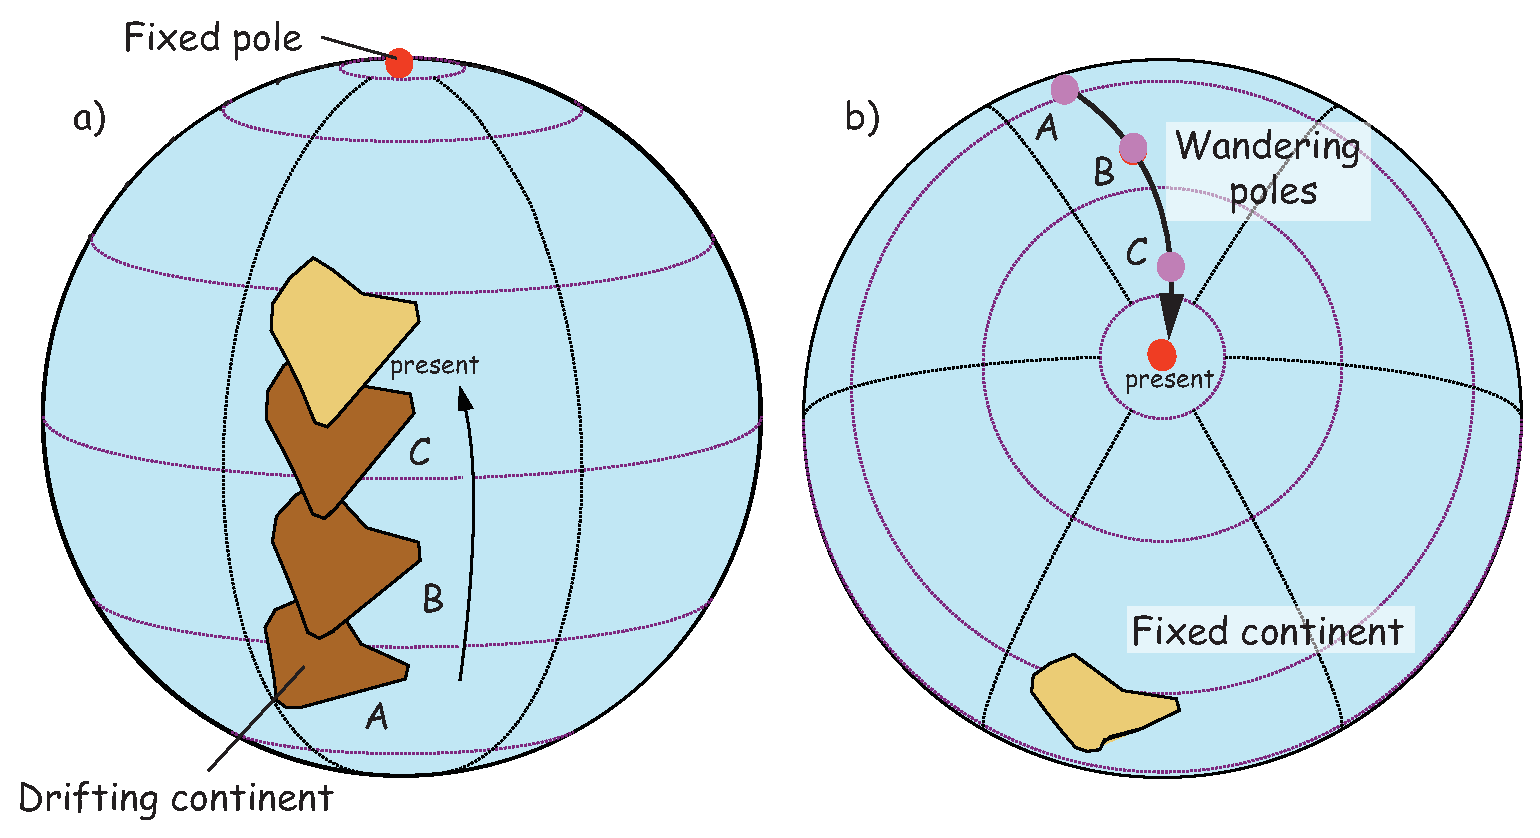
\includegraphics[width= 11.5 cm]{EPSfiles/wandering.eps}
\caption{  a) A moving continent will retain a record of changing paleomagnetic directions through time that reflect the changing orientations and distances to the pole (which is held fixed).  The resulting path of observed pole positions is called an ``apparent polar wander path'' or APWP because in this case the pole is actually fixed and only appears to move when viewed from the continental frame of reference.   b) On the other hand, if a continent is held fixed, the same changing paleomagnetic directions reflect the wandering of the pole itself.  This is called ``true polar wander'' or TPW.}
\label{fig:wandering}
\end{figure}

\index{plate tectonics}
\section  {Essentials of plate tectonic theory}

Well after the concept of continental drift and apparent polar wander had been accepted by most of the paleomagnetic community, the idea of sea-floor spreading and plate tectonics was developed to explain it.  In plate tectonics, the hard outer shell of the Earth, the {\it lithosphere}  is composed of many rigid or semi-rigid plates, the most important of which are shown in Figure~\ref{fig:plates}.     These plates are in constant motion with respect to one another.  The relative motion of two plates can be described by  rotation about an Euler rotation vector, which is usually specified by a pole latitude/longitude on the surface of the Earth ($\lambda_{e},\phi_e$) and a rotation rate $\omega$ in $^{\circ}$Myr$^{-1}$.  The velocity $v$ at a given point  on a plate with respect to its ``fixed'' partner varies as a function of angular distance from the Euler pole ($\theta$) as:

\begin{equation}
 v = a \omega \sin \theta,
 \label{eq:spreadingrate}
 \end{equation}
 
\noindent where $a$ is the radius of the Earth as in Chapter 2.     As an example, we show the motion of North America (NAM) with respect to ``fixed'' Europe (EUR) in Figure~\ref{fig:plates}b.  For simplicity, we have rotated the reference frame such that the current Euler pole
\index{DeMets, C.}
 (DeMets et al., 1994) \nocite{demets94}as the square.  Lines of co-latitude correspond to     $\theta$ in this projection, so the velocities  (usually expressed in cm/yr; see black arrows in Figure~\ref{fig:plates}b) increase away from the pole, with a maximum at $\theta = 90^{\circ}$. Beyond 90$^{\circ}$ the velocities decrease to the antipode of the Euler pole.   Spreading rates can be determined from marine magnetic anomalies and  their variation along the ridge crest can be fit with Equation~\ref{eq:spreadingrate} to find both $\omega$ and $\theta$, and helping to constrain the location of the Euler pole.


\begin{figure}[htb]
%\epsfxsize 14cm
%\centering \epsffile{EPSfiles/plates.eps}
\centering  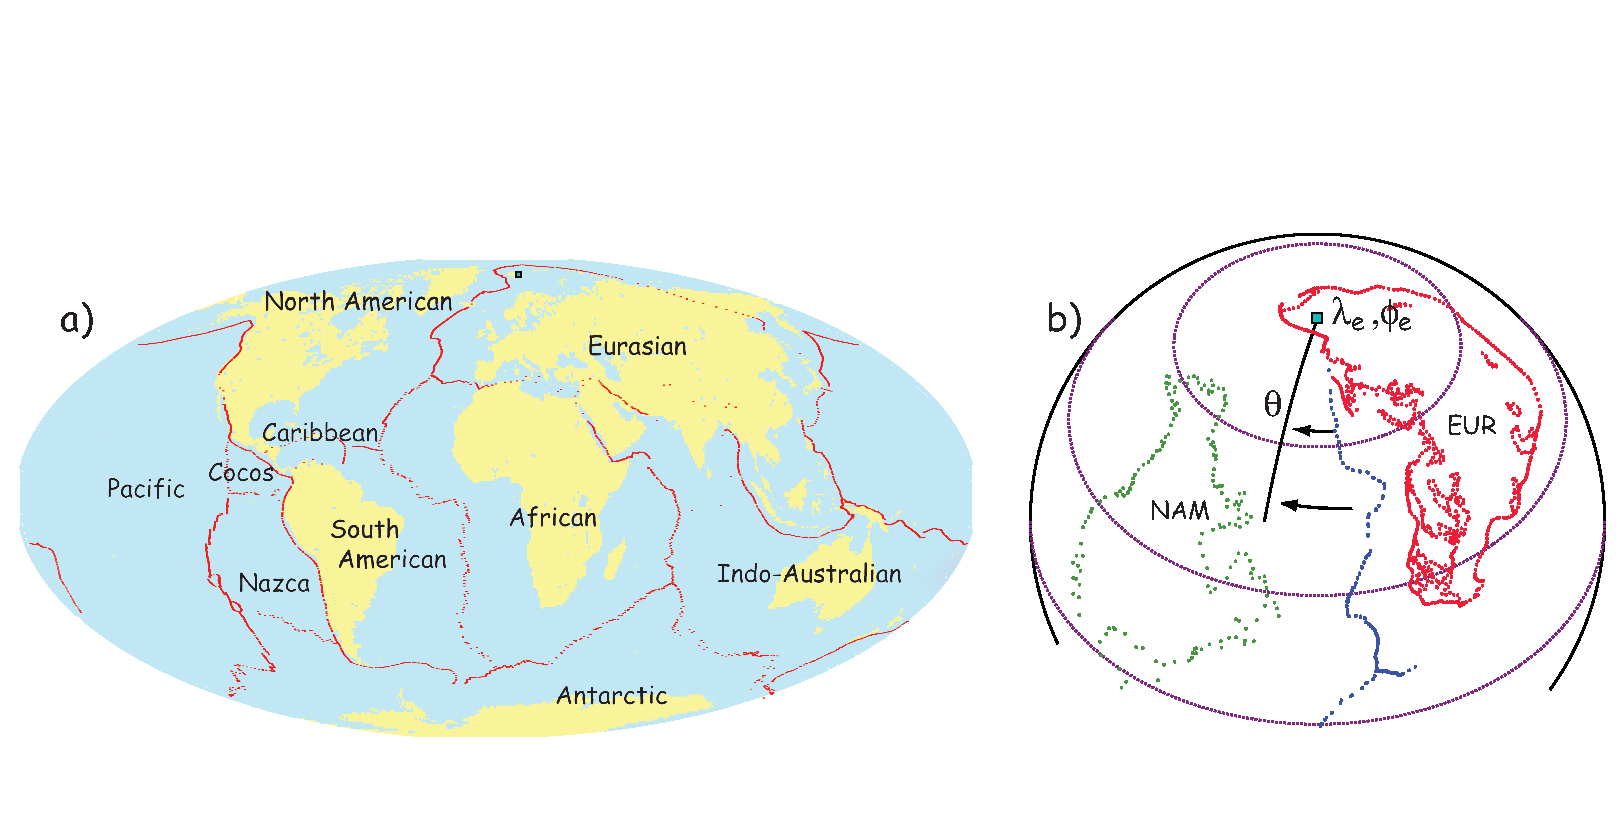
\includegraphics[width= 14 cm]{EPSfiles/plates.eps}
\caption{a) Some of the major lithospheric plates.  b) Motion of North America with respect to Europe around the Euler pole shown as a blue square.  Projection is such that current Euler pole North America (NAM) with respect to Europe (EUR) is at the ``North pole''.  Lines of co-latitude are the angular distance from the Euler pole, $\theta$.  Velocities of NAM with respect to EUR at two points with different $\theta$ are shown as black arrows.  }
\label{fig:plates}
\end{figure}


\begin{figure}[htb]
%\epsfxsize 14.5cm
%\centering \epsffile{EPSfiles/finrot.eps}
\centering  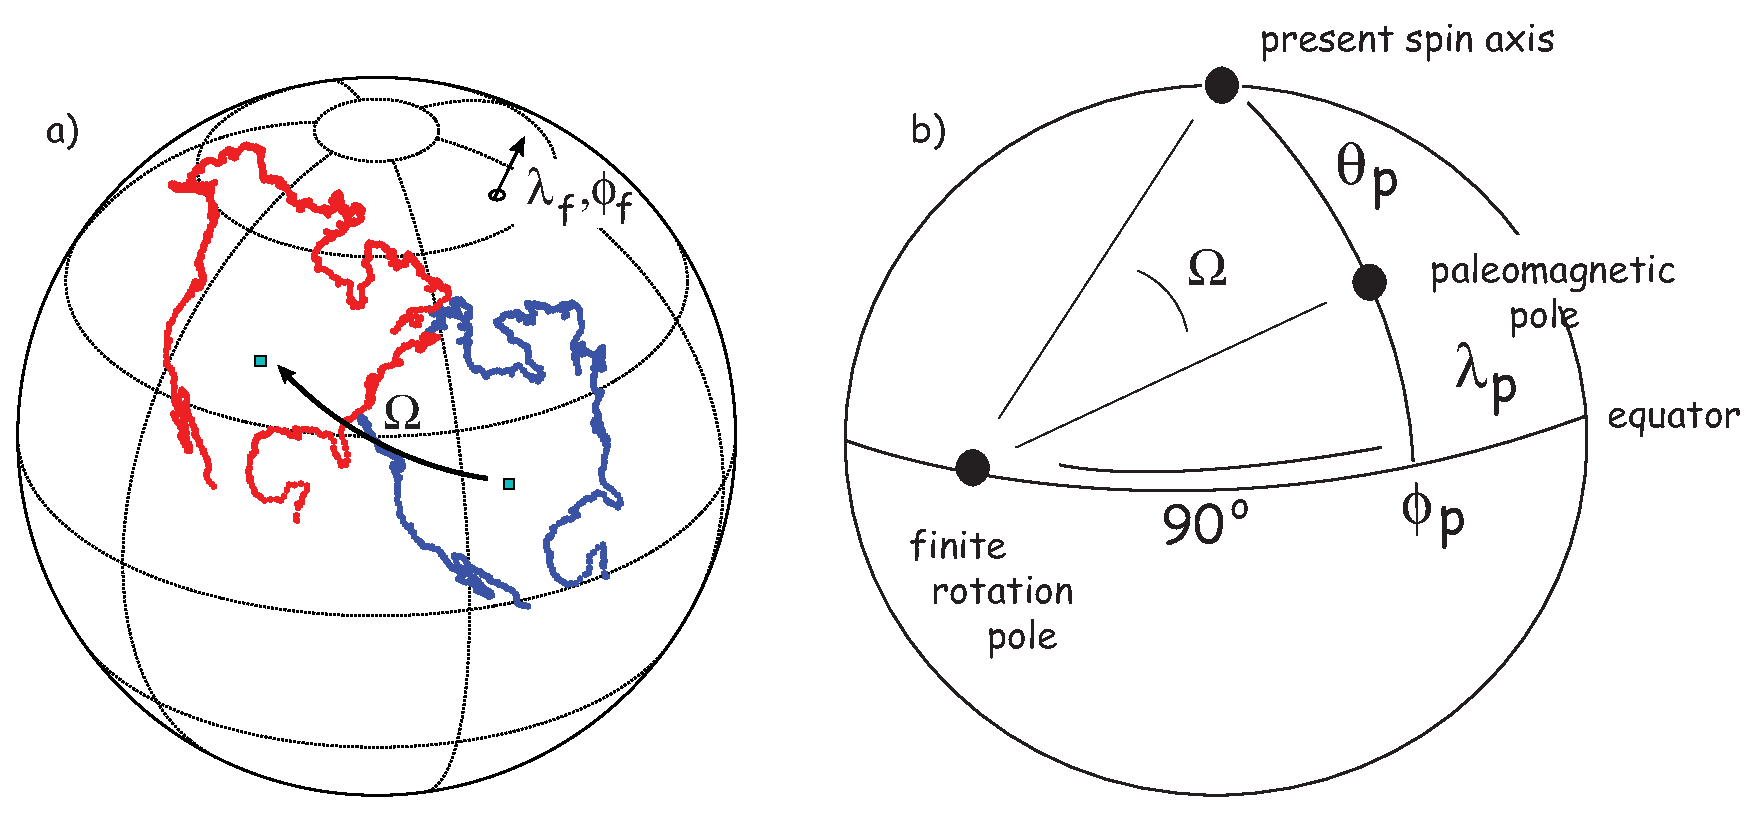
\includegraphics[width= 14.5 cm]{EPSfiles/finrot.eps}
\caption{a) Finite rotation of North America from one frame of reference to another.  Finite rotation pole is located at $\lambda_f,\phi_f$ and the finite rotation is $\Omega$. b) Estimating a finite rotation of a continental fragment  from a paleomagnetic pole.}
\label{fig:finrot}
\end{figure}


\index{Euler rotations}
Euler poles describe instantaneous rates of rotation of one plate or continental fragment with respect to another.  Often, what is known is not the rate, but the total rotation about a given pole that restores a plate to some prior state  (see Figure~\ref{fig:finrot}a.)  Such a pole is called a 
\index{finite rotation poles}
{\it finite rotation pole}.  
These   can be found in several ways.  Transforms and ridges define plate boundaries between two lithospheric plates and   are to first order perpendicular and parallel to the direction of the finite rotation pole respectively.   Marine magnetic anomalies  can also be restored to the spreading centers via finite rotations. Also, a finite rotation can be found that restores a position defined for example by the continental margins (e.g., the 
\index{Bullard fit}
{\it Bullard fit}  of the Atlantic bordering continents, 
\index{Bullard, E.C.}
 Bullard et al., 1965) or that maximizes agreement of paleomagnetic poles after rotation.  \nocite{bullard65}

   Tremendous effort has been put into compiling finite rotations for various lithospheric plates through time.  The most recent and comprehensive compilation is that of
   \index{Torsvik, T.H.}
Torsvik et al. (2008), \nocite{torsvik08} which goes back more than 300 Myr.   Reconstructions for the last 200 Ma are based mostly on marine geophysical data like marine magnetic anomalies, spreading center and transform azimuths, etc.  Pressing back in time, we run out of sea-floor when the Atlantic Ocean is completely closed and finite rotations between blocks must be constrained in  other ways, for example, fit of geological observations or paleomagnetic poles.  
Therefore finite rotations for times prior to about 200 Ma are not independent of the paleomagnetic pole data themselves.  Nonetheless, they provide a useful straw man frame of reference.  We include a partial list of finite rotations  in  Appendix~\ref{app:polerot}.    Details of how to rotate points on the globe using finite rotations are given in Appendix~\ref{app:polerot}, a technique that will be used extensively in this chapter.  


Defining finite rotations based on paleomagnetic poles finds a pole of rotation that transforms  the paleomagnetic poles observed on  continents back to the spin axis.  There are multiple possible finite rotations that achieve this and the problem is inherently non-unique.  We show one simple example in Figure~\ref{fig:finrot}b.     The latitude ($\lambda_{f}$) and longitude ($\phi_{f}$) of a finite pole of rotation can be found from a specified paleomagnetic pole ($\lambda_p, \phi_p$) by:

$$\lambda_f = 0, \phi_f = \phi_p - 90^{\circ}, \Omega = \theta_p.$$

\noindent  In this way, the points defining a particular continental fragment can be reconstructed to a position consistent with the paleomagnetic pole position; see for example, Figure~\ref{fig:wandering}a, which is in fact a series of reconstructions of the Indian subcontinent consistent with paleomagnetic poles determined at intervals for the last  80 Ma.  


 
 
 \begin{figure}[htb]
%\epsfxsize6cm
%\centering \epsffile{EPSfiles/polarity.eps}
\centering  \includegraphics[width= 6 cm]{EPSfiles/polarity.eps}
\caption{Polarity and paleolongitude can be ambiguous from paleomagnetic data alone.  All three  positions of the continental fragment (a,b,c) could be reconstructions of  the same observed direction.   a) and b) differ with assumed polarity.  b) and c) differ with assumed longitude.}
\label{fig:polarity}
\end{figure}


There are two problems with using paleomagnetic poles for constraining finite rotations, however.   The first arises from the fact that the  paleomagnetic field has two stable states. The two positions labeled a) and b) in Figure~\ref{fig:polarity} could have directions that are identical, but the polarity of the observed directions would be opposite.  If one had just a snap shot of one of these, without the context tying a particular direction to the North or South pole, it would be impossible to know which was the North seeking direction.  In recent times, this is not a problem because such a context exists, but in the Precambrian and early Paleozoic, the context can be lost and the polarity can be ambiguous.  The second problem with using paleomagnetic poles for constraining finite rotations is that paleo-longitude cannot be constrained from the pole alone;  the two positions labelled b) and c) in Figure~\ref{fig:polarity} are equally well fit by a given paleomagnetic pole.     




\section {Poles and apparent polar wander}
\label{sect:apwp}

 There have been over  10,000 paleomagnetic poles published since 1925.  These range in age from the Archean to quite recent and  in quality from excellent to highly questionable.  Paleomagnetic poles were assembled into the IAGA
  \index{databases!GPMDB}
Global Paleomagnetic  Database 
 (GPMDB)  accessible at Norwegian Geological Survey ({\it Dragon Project})  website: 
 
  \center \url{http://www.ngu.no/geodynamics/gpmdb/}
  
  \noindent  which allows searching by pole number (RESULTNO), age, geographic limits,  author, etc.


  \begin{figure}[htb]
%\epsfxsize 11cm
%\centering \epsffile{EPSfiles/poles-aus.eps}
\centering  \includegraphics[width= 11 cm]{EPSfiles/poles-aus.eps}
\caption{Paleomagnetic poles from Australia for the last 200 Ma from GPMDB. a) No selection criteria.  b) The selection criteria of BC02.}
\label{fig:poles.aus}
\end{figure}

%\customlink{apparent_polar_wander_path}
The goal of much paleomagnetic research has been to assemble the various poles or some subset  of poles into 
\index{apparent polar wander path}
{\it apparent polar wander paths}  (APWPs) for the many different continental fragments.    There are two  issues that guide the construction of APWP:  selection of poles which can be considered ``reliable'' and curve fitting.   

 Picking out the meaningful poles from the published data is part of the art of paleomagnetism.  We have been building a tool kit for dealing with this problem throughout this book.    \nocite{voo90} There is some agreement in  what constitutes a ``good'' pole   among various workers.  The general selection criteria used by most paleomagnetists  are based  on those  summarized  by 
 \index{van der Voo, R.}
 van der Voo (1990;V90).  They have been  modified for particular applications, for example, by 
 \index{Besse, J.}
 \index{Courtillot, V.} \nocite{besse02}
 Besse and Courtillot (2002; BC02) as noted in the following.  
 
 
\begin{enumerate}

\item The age of the formation must be known rather accurately.  In the V90 criteria, the age should be known to within a half of a geological  period (see Chapter 15) or within a numerical age of $\pm$ 4\% for Phanerozoic data.  For Precambrian rocks, the age should be known to within $\pm$ 4\% or 40 Myr, whichever is smaller.  Some applications require that poles be rotated from one continental reference frame to another, which demands tighter age constraints. For example,  BC02\nocite{besse02} set age uncertainties of  $< \pm$ 15 Myr.  

\item  In order to average errors in orientation of the samples 
and scatter caused by
secular variation, there must be a sufficient number of
 individually oriented samples from
enough sites.  What constitutes
``sufficient" and ``enough" here is somewhat subjective and a matter
of debate. 
The V90 Criteria recommend a minimum of 24 
discrete samples of the geomagnetic field each having a 
$\kappa>10$. Some authors also compare scatter within and between sites 
in order to assess  whether secular variation has been sufficiently sampled, but
this relies on many assumptions as to what the magnitude of secular variation   was (see Chapter 14).  
\index{Butler, R.F.}
Butler (1992) \nocite{butler92} suggested using the scatter of VGPs ($S_p$ in Chapter 14)  to decide whether secular variation has been averaged out or whether there is excess scatter in the data set.    BC02 recommend using  only poles with at least six sites and 36 samples, each site  having a 95\% confidence interval less than 10$^{\circ}$ in the Cenozoic and 15$^{\circ}$ in the Mesozoic.    

\item  It must be demonstrated that a coherent
characteristic remanence component has been isolated by the
demagnetization procedure.     
\index{McElhinny, M.W.}
\index{McFadden, P.L.}
McElhinny and McFadden (2000) \nocite{mcelhinny00} attempted to standardize the description of the demagnetization status of a dataset using a demagnetization code (DC) (see  Table~\ref{tab:DC}).     BC02 recommend using only poles with a DC of at least 2.

\item  The age of the magnetization relative to the age of the rock
 should be constrained using field tests (fold test, conglomerate test, baked contact test, see Chapter 9).   BC02 reject poles that fail a fold test or a reversals test.  

\item  There should be agreement in the pole positions from
  units of similar age from a broad region and adequate knowledge of any structural corrections necessary.    BC02 reject poles from ``mobile regions'', but incorporate data that are azimuthally unconstrained by using  inclination only data  as a constraint on paleolatitude  (see Section~\ref{sect:inconly} for a more complete discussion).  
  
  \item Both polarities should be represented and the two data sets should be antipodal.  

\item  Pole positions should not  fall on a younger part of the 
pole path or on the present field direction. Such poles should be viewed with suspicion.

\end{enumerate}

 
 \begin{figure}[htb]
%\epsfxsize 14cm
%\centering \epsffile{EPSfiles/mkapwp.eps}
\centering  \includegraphics[width= 14 cm]{EPSfiles/mkapwp.eps}
\caption{Examples of how to construct an APWP.  a) Discrete window.  b) Key pole approach. c) Moving window (Besse and Courtillot, 2002) versus  spline (Torsvik et al.,  2008).  }
\label{fig:mkapwp}
\end{figure} \nocite{besse02} \nocite{torsvik08}




 In the V90 criteria, each pole gets a point for every criterion that it passes.   The sum of the points is the quality factor $Q$ which ranges from 0 to 7.    It is not expected that every pole satisfy all seven criteria (very few would!).  Most authors use poles with  $Q>2$.     BC02 on the other hand use criteria 1-5 (must have all of them) but do not require 6 or 7.




In order to understand the  process of constructing
\index{apparent polar wander path}
APWPs, we will  begin with the plot of  all the paleomagnetic poles from  Australia for the last 200 Myr (Figure~\ref{fig:poles.aus}).  
 These poles form a smear that extends in a broad arc away from the spin axis down the Atlantic and then into Europe and Africa.  
Of the 137 poles from Australia in the 
\index{databases!GPMDB} 
GPMDB plotted in Figure~\ref{fig:poles.aus}a, only 18 meet the BC02 criteria (see Figure~\ref{fig:poles.aus}b).   These form a sparse track which could form the basis for an APWP.  

  
Once selected, the poles must be combined together somehow in order to define an apparent polar wander path for any of  the continental fragments.  The goal of this process is to produce a list of paleomagnetic poles at more or less uniform time intervals for each independent lithospheric fragment.  There have been several different approaches to this problem in the literature as summarized below:  


\begin {enumerate}

\item Discrete windows  (Figure~\ref{fig:mkapwp}a):   Selected poles for a given continent or continental fragment are separated into discrete time intervals and poles in each   time window are averaged.  There is no overlap of poles between windows so each window is independent of the others.  

\item Key poles:   Practitioners identify what are considered to be the most reliable poles, so-called ``key poles''  (e.g., largest dots in Figure~\ref{fig:mkapwp}b).  If the data quality is highly uneven, key poles can be used as anchor-points. 


\item Moving windows:  Same as (1), but time windows overlap and paleopoles can be  included in more than one window. Successive mean poles are not independent of each other (see Figure~\ref{fig:mkapwp}c).


\item Fitting curves with splines:  This technique fits a smoothly curving path to the available paleopoles 
\index{Jupp, P.E.}
\index{Kent, J.T.}
(Jupp and Kent, 1987), some of which can be weighted more than others (see Figure~\ref{fig:mkapwp}c).
\nocite{jupp87}



 \begin{figure}[htb]
 %\epsfxsize 14.5cm
 %\centering \epsffile{EPSfiles/PEP.eps}
 \centering  \includegraphics[width= 14.5 cm]{EPSfiles/PEP.eps}
 \caption{a) Paleomagnetic Euler pole method for determining APWPs.   A continent is rotating about a fixed Euler pole (green triangle).  
As the continent moves, rocks record paleomagnetic directions reflecting the position of the spin axis at that particular age.  b) When viewed in the present coordinate system  and converted to paleomagnetic poles, these will 
 fall  on the small circle  APWP track.  c) PEP analysis for Jurassic APWP for North America of May and Butler (1986).  Poles are interpreted to lie along small circle tracks (J1/J2) separated by a cusp (J2 cusp) located at the LM pole. The J1 and J2 tracks are small circles about their respective Euler poles, shown as blue triangles.   }
 \label{fig:PEP}
 \end{figure}
 

\index{paleomagnetic!euler pole analysis}
\item PEP analysis: Paleomagnetic Euler Pole analysis assumes that APWP segments are small circles about an Euler pole 
\index{Gordon, R.G.}
(Gordon et al., 1984; see Figure~\ref{fig:PEP}a.) \nocite{gordon84} The underlying assumption is that the continents move according to the same Euler vector for  considerable stretches of time (e.g., $\sim$ 10$^7$ years).  When viewed from the continental frame of reference, the poles plot along an apparent polar wander path that forms a small circle about the Euler pole (Figure~\ref{fig:PEP}b).  
\index{May, S.R.}
\index{Butler, R.F.}
May and Butler (1986)  \nocite{may86} applied the technique to the North American APWP.  Their compilation of Jurassic key poles is shown in  Figure~\ref{fig:PEP}c.  These were interpreted to lie along two tracks (J1 and J2) separated by a cusp (J2 cusp) at the LM (Lower Morrison Formation) pole.  Each track is a small circle about its respective Euler pole (shown as blue triangles).  We will return to this topic in Section~\ref{sect:inconly}. 

\item Master path:  The ``master path'' approach (e.g., 
\index{Besse, J.}
\index{Courtillot, V.}
\index{Torsvik, T.H.}
Besse and Courtillot, 2002; Torsvik et al. 2008) argues that if the rotation parameters between continents are well known as a function of age, then poles from one continent can be transferred to the coordinate system of  another.  When all suitable poles  are transferred to a single continent they can be used to constrain a single synthetic apparent polar wander path by, for example, windowing or spline fitting.  The synthetic path can then be exported back to the contributing continents (see, e.g., Figure~\ref{fig:apwp}e).      


\item  Use of inclination only data from regions suspected of local rotations.  Even if a region has undergone local rotation, the inclinations provide constraints for paleolatitude.  The paleomagnetic pole must lie on the paleolatitude small circle  around the site location.    These small circles can be used to supplement fully oriented paleopoles, or if  there are enough data from sufficiently disparate locations, a unique intersection can be used to define the position of the paleomagnetic pole (see Figure~\ref{fig:triangulation}).   


  
\end{enumerate}







  \begin{figure}[htb]
%\epsfxsize 14cm
%\centering \epsffile {EPSfiles/APWP.eps}
\centering  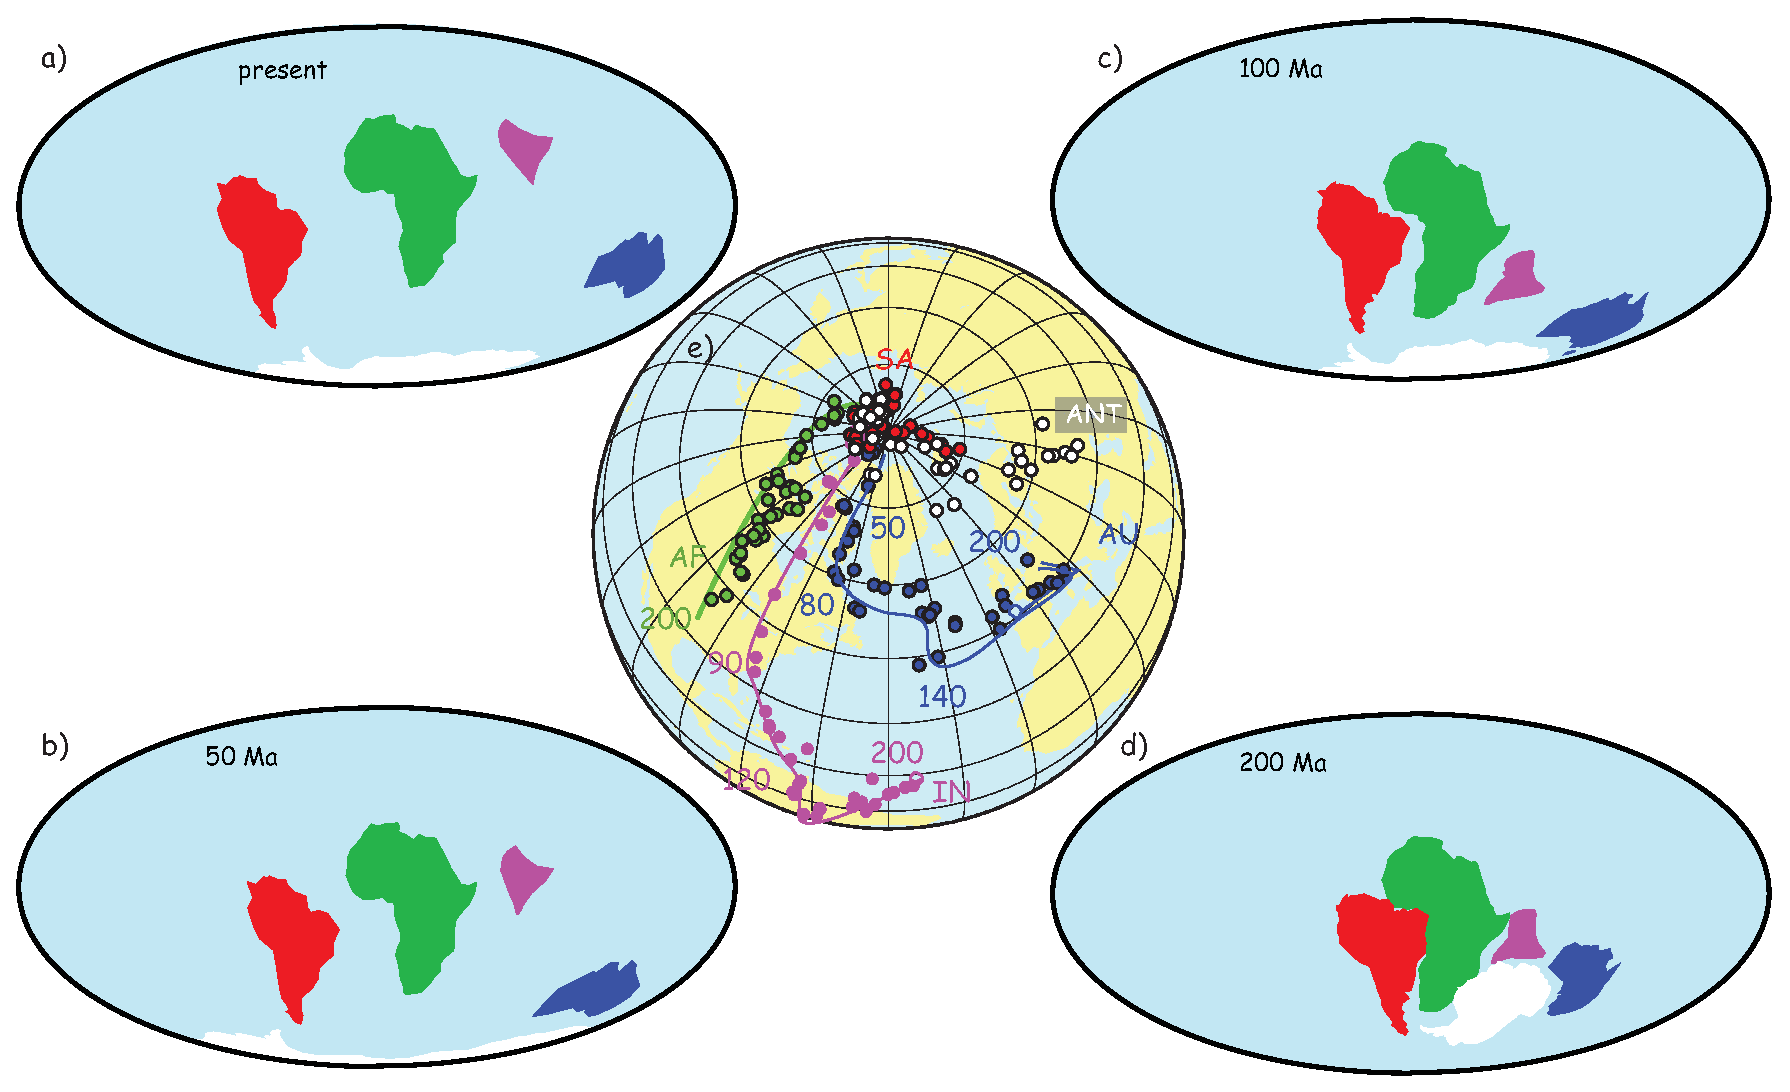
\includegraphics[width= 14 cm]{EPSfiles/APWP.eps}
\caption{
Master path approach:  Maps of continental reconstructions for a) present, b) 50, c) 100, and d) 200 Ma. e)  Poles and APWP for various continents for the last 200 million years, evaluated at five million year intervals.  [Reconstructions using finite rotation poles of Torsvik et al. 2008 (see Appendix~\ref{app:polerot}).]  Paleomagnetic poles from the synthetic APWP constructed by Besse and Courtillot, (2002) exported to the different continents. }
\label{fig:apwp}
\end{figure}  \nocite{torsvik08} \nocite{besse02}


  \begin{figure}[htb]
%\epsfxsize 6cm
%\centering \epsffile {EPSfiles/triangulation.eps}
\centering  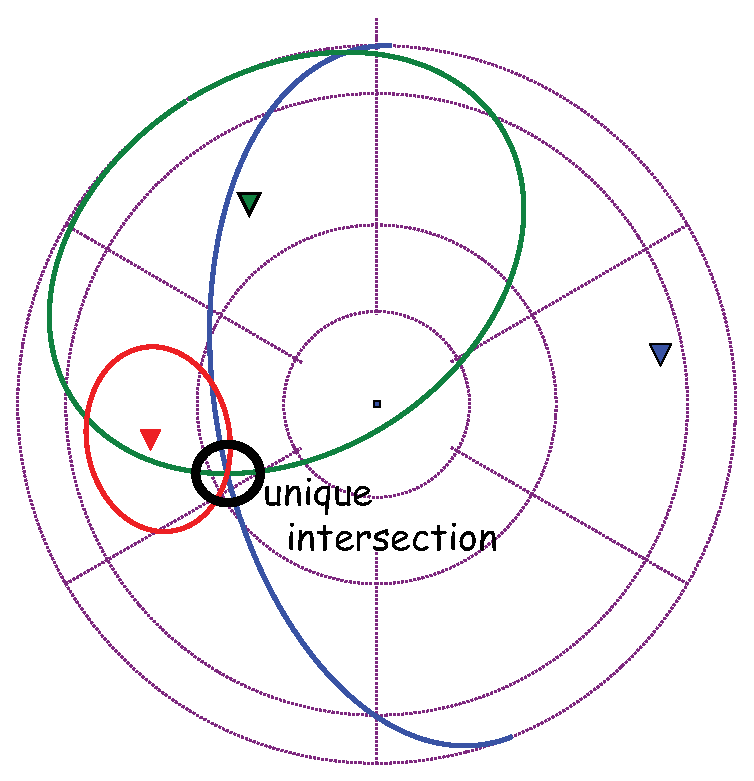
\includegraphics[width= 6 cm]{EPSfiles/triangulation.eps}
\caption{Sampling sites are marked by triangles.  Inclinations from the sites can be used to calculate the paleomagnetic colatitude of the site using the dipole formula (see Chapter 2) which defines a small circle along which the paleomagnetic pole must lie.  The intersection of three such small circles uniquely defines the position of the paleomagnetic pole.
}
\label{fig:triangulation}
\end{figure}



\begin{table}[h!]
\caption{Demagnetization Codes (DC) summarized by McElhinny and McFadden (2000).}
\label{tab:DC}
\begin{tabular}{ll}
\hline
DC & Description\\
\hline
0 & Only NRM values reported.  No evidence for demagnetization.\\
1 & Only NRM values reported.  Demagnetization on pilot \\
& \hskip 1em specimens suggest stability.\\
2 & Demagnetization at a single step on all specimens.  \\
& \hskip 1em No demagnetograms shown.\\
3 & Demagnetograms shown that justify demagnetization procedure chosen.\\
4 & Principal component analysis (PCA) carried out from analysis of  \\
& \hskip 1em Zijderveld diagrams. (see Chapter 9)\\
5 & Magnetic vectors isolated using two or more demagnetization  \\
& \hskip 1em methods with PCA.\\
& e.g.,  thermal and AF demagnetization (see Chapter 9). \\
\hline
\end{tabular}
\end{table}


 

\begin{figure}[htb]
%\epsfxsize 12cm
%\centering \epsffile{EPSfiles/gondwana-apwp.eps}
\centering  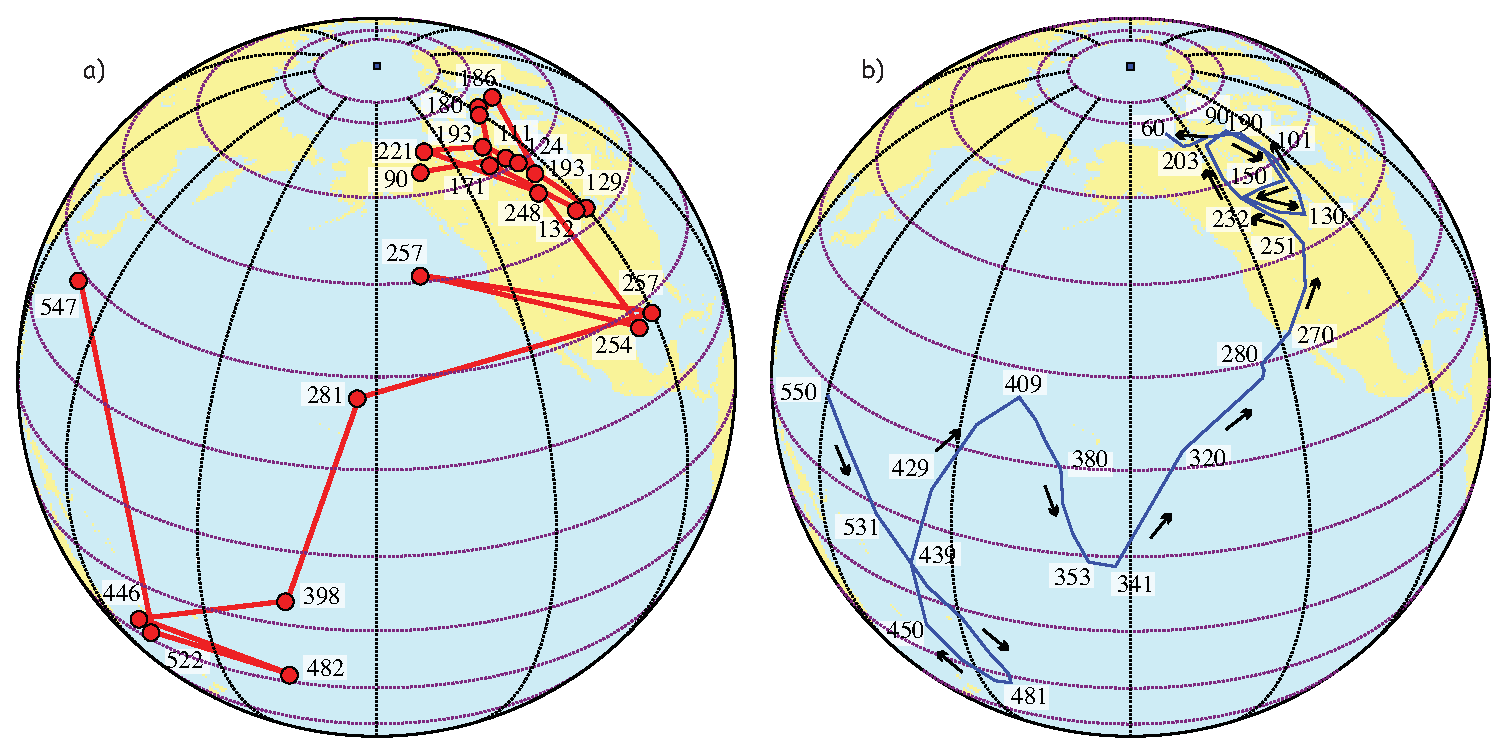
\includegraphics[width= 12 cm]{EPSfiles/gondwana-apwp.eps}
\caption{The South African APWP for the Phanerozoic.  a) South African poles only (Table 1 of Torsvik and van der Voo, 2002).  b) Smoothed APWP spline path using master path approach for Gondwana in South African coordinates. }
\label{fig:gondwana}
\end{figure}

\section{The Gondwana APWP}


\index{Besse, J.}
\index{Courtillot, V.}
Besse and Courtillot (2002) produced a master path for the last 200 Myr and 
\index{Torsvik, T.H.}
Torsvik et al. (2008) refined the poles of rotation and extended them back to 320 Ma.  Prior to about 200 Ma, however, rotation poles are more difficult to  constrain, independent of the paleomagnetic data themselves.   Both the quality and quantity of the available poles decline with increasing age.    The assumptions of the GAD hypothesis and amount and style of secular variation become increasingly problematic.    Furthermore, most continents are composed of separate blocks whose relationships in ancient times are unknown or poorly known.  Exceptions to this are supercontinents like Gondwana  for which it is possible to combine data from different blocks with some confidence.    


Gondwana was a supercontinent that coalesced about  550 Ma and was incorporated into a larger supercontinent of Pangea during the Carboniferous.  Pangea itself began breaking up during the Mid-Jurassic when the Atlantic Ocean began to form.   The core continental fragments that comprise Gondwana are NE, NW and Southern Africa, South America, Madagascar, Greater India, Cratonic Australia and East Antarctica.
\index{Torsvik, T.H.}
\index{van der Voo, R.}
Torsvik and van der Voo (2002) \nocite{torsvik02} compiled a list of paleomagnetic poles from these core parts of the Gondwana continents ($Q\ge3$ for the V90 criteria)  along with a  set of finite rotation poles for putting them back together.

As an example of the kind of pole paths available for an individual continent, we show all the poles selected by 
\index{Torsvik, T.H.}
\index{van der Voo, R.}
Torsvik and van der Voo (2002) from the South African continental fragment in Figure~\ref{fig:gondwana}a.  The inferred path is quite complicated in the Mesozoic and  the poles are sparse prior to about 250 Ma  leading to the suspicion that the path is somewhat undersampled.  
 By rotating poles from all the Gondwana continental fragments into South African coordinates and fitting them with a smoothed path using splines,  Torsvik and van der Voo (2002) produced the 
 \index{apparent polar wander path}
 APWP shown in Figure~\ref{fig:gondwana}b.  
 
 Pushing back to times before Gondwana gets increasingly difficult because indigenous poles become more sparse and more poorly dated and reconstruction of the pre-Gondwana continental bits becomes less well constrained.    Nonetheless, some authors have pushed their interpretations of Cambrian data reach rather extreme conclusions.  For example, large swings in the APWP for Australia led to the conclusion that the entire spin axis of the Earth changed by 90$^{\circ}$ suddenly in a feat termed ``inertial interchange true polar wander'' (see, e.g.,
 \index{Kirschvink, J.}
  Kirschvink et al., 1997).  \nocite{kirschvink97b}


 
\begin{figure}[htb]
%\epsfxsize 14cm
%\centering \epsffile{EPSfiles/squish.eps}
\centering  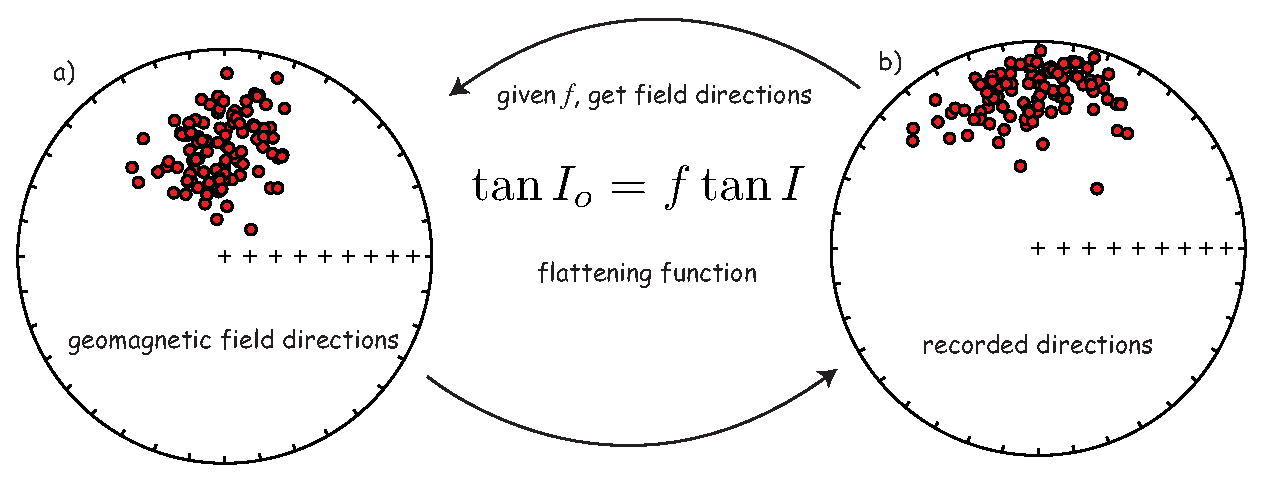
\includegraphics[width= 14 cm]{EPSfiles/squish.eps}
\caption{a) Set of possible geomagnetic field directions plotted in equal area projection.  Lower (upper) hemisphere directions  are solid (open) symbols.   b) Directions recorded by the sediment using the flattening function.  [Figure modified from Tauxe et al., 2008] }
\label{fig:squish}
\end{figure} \nocite{tauxe08,tauxe84}




\section{Inclination shallowing and GAD}
\label{sect:tk03}

One of the most useful, in fact essential,  assumptions in paleomagnetism is that the geomagnetic field is on average closely approximated by a geocentric axial dipole (GAD).  As discussed in Chapter 14, the GAD hypothesis has been found to be nearly true for at least the last 5 million years with the largest non-GAD contribution to the spherical harmonic expansion generally being of the order of 5\%.  For the more ancient past, it is difficult to test the GAD (or any other field) hypothesis owing to plate motions, accumulating problems of overprinting, and difficulty in reconstructing paleo-horizontal. Although most paleomagnetic studies make the implicit assumption of a GAD field, several recent studies have called the essential GAD nature of the ancient field into question. These studies fall into two groups: those that use reference poles and plate tectonic reconstructions to predict directions (e.g., 
\index{Si, J.}
\index{van der Voo, R.}
Si and van der Voo, 2001) \nocite{si01} and those that compare observed  statistical distributions of directions to those predicted by different field models (e.g.,
\index{Kent, D.V.}
\index{Smethurst, M.A.}
 Kent and Smethurst, 1998; van der Voo and 
\index{Torsvik, T.H.}
 Torsvik, 2001). \nocite{kent98} \nocite{voo01} The inescapable conclusion from these and other studies is that there is often a strong bias toward shallow inclinations and many studies have called on  non-dipole field contributions, in particular large  (up to 20\%) average zonal octupole ($g_3^0$) contributions (see Chapters 2 and 14).   We will explore these ideas in the following.
\nocite{voo81}

\nocite{gilder01,tauxe04d}
\begin{figure}[htb]
%\epsfxsize 14.5cm
%\centering \epsffile{EPSfiles/EI.eps}
\centering  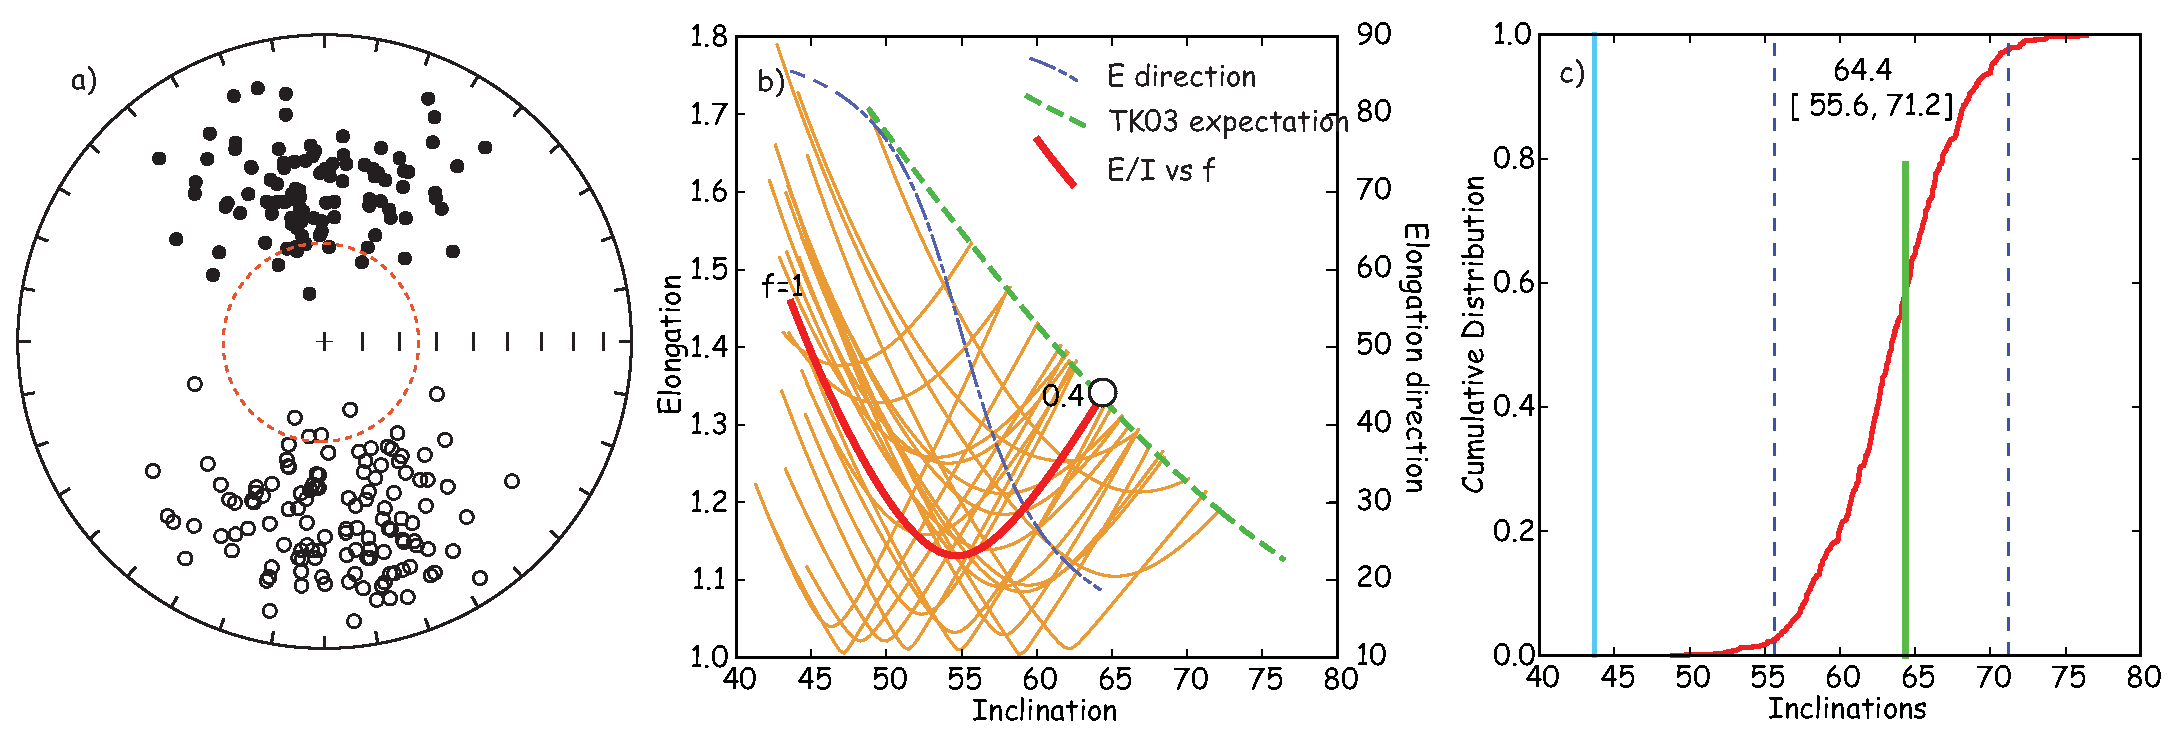
\includegraphics[width= 14.5 cm]{EPSfiles/EI.eps}
\caption{a) Paleomagnetic directions of Oligo-Miocene redbeds from Asia  in equal area projection (stratigraphic coordinates). [Redrawn from Tauxe and Kent, 2004; data from Gilder et al., 2001.]. b) Plot of elongation versus inclination for the data  (heavy red line) and for the TK03.GAD model (dashed green line).  Also shown are results from 20 bootstrapped datasets (yellow).  The crossing points represents the inclination/elongation pair most consistent with the TK03.GAD model.   Elongation direction is shown as a dash-dotted (purple) line and ranges from E-W at low inclination to more N-S at steeper inclinations.  c) Cumulative distribution of crossing points from 5000 bootstrapped datasets.   The inclination of the whole data set (64.4$^{\circ}$) is consistent with that predicted from the {{\it} Besse and Courtillot } (2002)  European APWP. The 95\% confidence bounds on this estimate are 55.6-71.2$^{\circ}$. }
\label{fig:EI}
\end{figure}

%\customlink{TK03}
From Chapter 14 we know that paleomagnetic directions from the last five million years are, if anything, elongate in the North-South vertical plane.  However,  sedimentary inclination flattening not only results in directions that are too shallow, but also reduces N-S elongations  in favor of elongations that are more east-west.   This effect is shown in Figure~\ref{fig:squish}.  
Geomagnetic field directions (e.g., Figure~\ref{fig:squish}a)  with inclinations $I_f$ are recorded in sediments with  observed inclinations ($I_o$) following the  flattening function  of 
\index{King, R.F.}
King (1955) \nocite{king55} (see Chapter 7),  $\tan I_o = f \tan I_f$, where  $f$ is the flattening factor ranging from unity (no flattening) to 0 (completely flattened).  Examples of the recorded  ``flattened'' directions are shown in Figure~\ref{fig:squish}b.    Note that flattened directions tend to become elongate in the horizontal plane, a feature that distinguishes this cause of inclination shallowing from others, for example, poleward plate motion which leaves the distribution unchanged or non-dipole field effects.  Zonal non-dipole field contributions like those from axial quadrupole or octupole fields make the distribution more elongate in the meridional plane (see, e.g., 
\index{Tauxe, L.}
\index{Kent, D.V.}
Tauxe and Kent,  2004).  
 \nocite{tauxe04d}



Earlier in the chapter, we discussed the BC02 APWPs for the major continents.  These can be used to predict directions for a given time and place using the spherical trigonometric tricks covered in Appendix~\ref{app:strig}.    Despite the general success of the BC02 APWPs for predicting directions, comparison of predicted directions with those observed in many data sets from red beds in Central Asia led some authors to the conclusion that the GAD hypothesis had failed.   We show an example of such a data set in Figure~\ref{fig:EI}a, although it is atypical in that there are an unusually  large number of directions.  These  have a mean of $\bar D$ = 356.1$^{\circ}$, $\bar I$ =43.7$^{\circ}$.  Assuming that the location of the study (presently at 39.5$^{\circ}$N, 94.7$^{\circ}$E)  has been fixed to the European coordinate system and taking the 20 Myr pole for Europe from \nocite{besse02} BC02 (81.4$^{\circ}$N, 149.7$^{\circ}$E), the inclination  is predicted to be 63$^{\circ}$  (see dashed curve in Figure~\ref{fig:EI}a).  These sediments are typical of Asian sedimentary units in having an  inclination relative to the predicted values that is some 20$^{\circ}$ too shallow.  


\index{inclination!error!correction of!elongation-inclination method}
The 
{\it elongation-inclination} (E/I) method of detecting and correcting inclination shallowing  of Tauxe and Kent (2004, see also Tauxe et al., 2008) \nocite{tauxe04d,tauxe08} simply ``unflattens'' observed directional data sets using the inverse of the flattening formula and values for $f$ ranging from 1 (no unflattening) to 0.4.  At each unflattening step, we calculate inclination and elongation ($\tau_2/\tau_3$ of the orientation matrix, see Appendix~\ref{app:eigen})  and plot these as in Figure~\ref{fig:EI}a.   We know from Chapter 14 that elongation decreases from the equator to the pole, while inclination increases; A  best-fit polynomial through the  inclination - elongation data from model TK03.GAD  is: $E= 2.895 - 0.01466 I - .0004 I^2$ (as recalculated by 
\index{Tauxe, L.}
Tauxe et al., 2008) \nocite{tauxe08} and  is shown as the green  line in Figure~\ref{fig:EI}b.  There is a unique pair of elongation and inclination that is consistent with the TK03.GAD field model (circled in Figure~\ref{fig:EI}b) with an inclination of 64$^{\circ}$.  As $f$ goes from 1 to 0.4, the inclination of the unflattened directions increases from about 45$^{\circ}$ to about 65$^{\circ}$.  At the same time the direction of elongation (dash-dotted  line -- see right hand vertical axis label) changes systematically from East-West ($\sim$85$^{\circ}$) to more North-South ($\sim$15$^{\circ}$).  


\begin{figure}[htb]
%\epsfxsize 14cm
%\centering \epsffile{EPSfiles/pangea.eps}
\centering  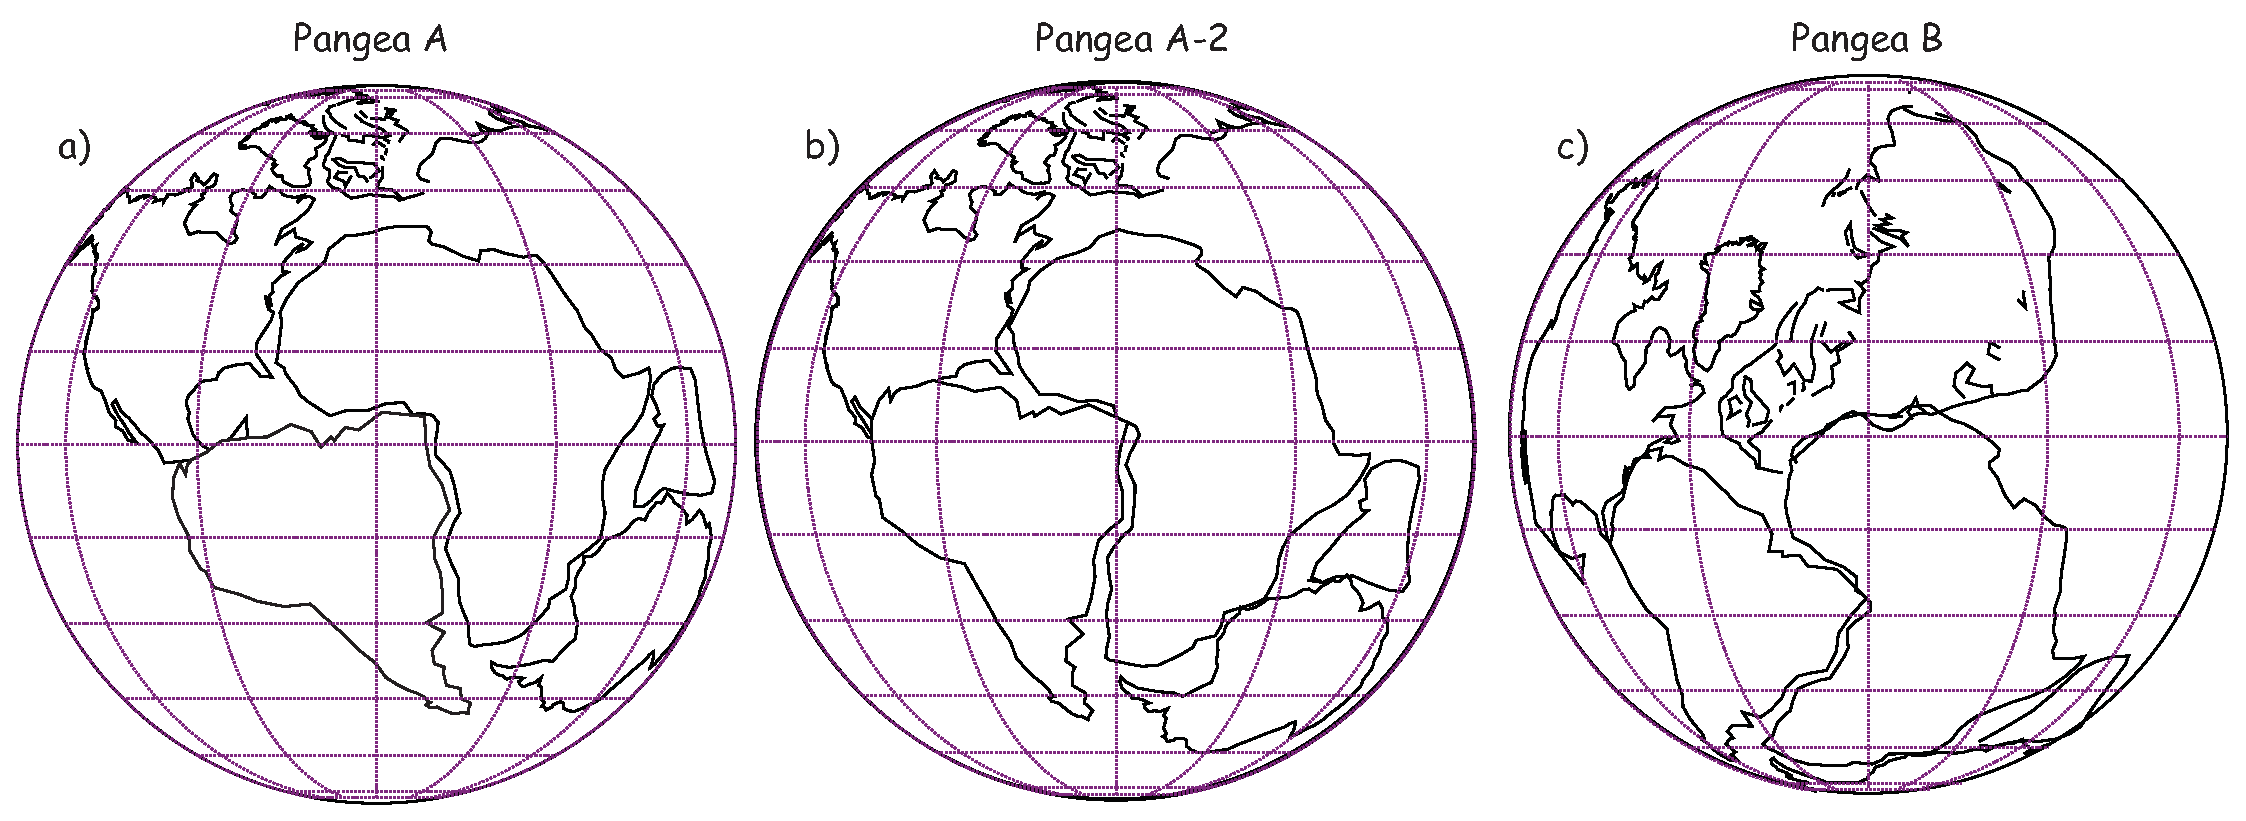
\includegraphics[width= 14 cm]{EPSfiles/pangea.eps}
\caption{a) Pangea A reconstruction (``Bullard fit''; Smith and Hallam, 1970), Bullard et al., 1965).  b) Pangea A-2 reconstruction (van der Voo and French, 1974).  c) Pangea B reconstruction (Morel and Irving, 1981).   Note: a) and b) are reconstructions to fit the continental margins and do not take into account paleolatitudes.   }
\label{fig:pangea}
\end{figure}
\nocite{smith70,bullard65,voo74,morel81}



 To obtain confidence bounds on the ``corrected'' inclination, the E/I method performs a bootstrap (see Appendix~\ref{app:bootstrap}).  
E/I curves from twenty such  bootstrapped data sets are shown as thin lines in Figure~\ref{fig:EI}b.  A cumulative distribution curve of 5000 crossing points of bootstrap  curves with the model elongation-inclination line are plotted in Figure~\ref{fig:EI}c.  The average inclination of the original (uncorrected) data is shown as the  light blue line in the plot and the corrected inclination as the heavy green line at 64.4$^{\circ}$.  The  95\% confidence bounds are shown as dashed lines at  55.6 and 71.2$^{\circ}$. The E/I corrected inclination is  consistent with that predicted by the BC02 path for stable Europe.    

\index{Tan, X.D.}
Tan et al. (2003) \nocite{tan03} performed the AARM correction (see Chapter 13) on the Tarim red beds and found a similar correction factor.  Hence  AARM correction (which is labor intensive in the lab) and EI correction (which is labor intensive in the field) give similar results.  Both methods strongly suggest that inclination shallowing in the Asian red beds is indeed caused by sedimentary inclination shallowing of the type described in Chapter 7. 

\begin{table}[htb]
\caption{Rotation poles for various versions of Pangea.}
\label{tab:pangea}
\begin{tabular}{|r|rrr|rrr|rrr|rrr|rrr|}
\hline
\multicolumn{16}{|c|}%
{Gondwana Continents:}\\
\hline
\multicolumn{16}{|c|}%
{Pangea A: Bullard et al. (1965), Smith and Hallam (1970)}\\
\hline
&&AF&& & AUS &  &  & ANT &  &  & IND  & & &SAM&\\
\hline
\# & $\lambda$ & $\phi$ & $\Omega$ & $\lambda$ & $\phi$ & $\Omega$ & $\lambda$ & $\phi$ & $\Omega$ & $\lambda$ & $\phi$ & $\Omega$ & $\lambda$ & $\phi$ & $\Omega$\\ 
 \hline
1&&&&-4&40&-31&1& -36 &58&29&42&-59&44&-31&57\\
2 &0&0&0& 1&-36&58 &&&&&&&&&\\
\hline
\multicolumn{16}{|c|}%
{Pangea A-2: van der Voo and French (1974)}\\
\hline
1&&&&-4&40&-31&1& -36&58&29&42&-59&44&-31&57\\
2 &&&& 1&-36&58&&&&&&&&&\\
3 &19 &-1&-20&19 &-1&-20&19 &-1&-20&19 &-1&-20&19 &-1&-20\\
\hline
\multicolumn{16}{|c|}%
{Pangea B: Morel and Irving (1981)}\\
\hline
1&&&&-4&40&-31&1& -36 &58&29&42&-59&44&-31&57\\
2 &&&& 1&-36&58 &&&&&&&&&\\
3&0&147&50&0&147&50&0&147&50&0&147&50&0&147&50\\
\hline
\multicolumn{16}{|c|}%
{Laurasian Continents:}\\
\hline
\multicolumn{16}{|c|}
{Pangea A: Bullard et al. (1965), Smith and Hallam (1970)}\\
\hline
&&&&&NAM&& & EUR&&&GRN &&&&\\
\hline
\# &&&& $\lambda$ & $\phi$ & $\Omega$ & $\lambda$ & $\phi$ & $\Omega$ & $\lambda$ & $\phi$ & $\Omega$&&& \\ 
 \hline
1&&&&68&-14&75&89&28&-38&73&97&22&&&\\
2&&& &&&& 68&-14&75&89&28&-38&&&\\
3&&&&&&&&&&68&-14&75&&&\\
\hline
\multicolumn{16}{|c|}%
{Pangea B: Morel and Irving (1981)}\\
\hline
 \hline
 
1&&&&68&-14&75&89&28&-38&73&97&22&&&\\
2&&& &&&& 68&-14&75&89&28&-38&&&\\
3&&&&&&&&&&68&-14&75&&&\\
4&&&&0&129&47&0&138&58&0&129&47&&&\\
5&&&&-90&0&31&-90&0&36&-90&0&31&&&\\
\hline
\end{tabular}
\#: Rotation number.  Rotations performed in order using algorithm in Appendix~\ref{app:polerot}.   $\lambda, \phi, \Omega$ are the latitude, longitude and angle of the finite rotation pole.  AF: Africa, AUS: Australia, ANT: East Antarctica, IND: India, SAM: South America, NAM: North America, EUR: Europe and GRN: Greenland.  
\end{table}

 \begin{table}[htb]
 \caption{ Paleomagnetic data for Kimmeridgian. }
 \label{tab:inconly}
\begin{tabular}{llllllllll}
\hline
Name & Age (Ma) &Plate&$S_{\lambda}(^{\circ}$N)&$S_\phi(^{\circ}$E)& $P_{\lambda}$& $P_\phi$&$P_{\lambda}^{AF}$ & $P_{\phi}^{AF}$ & Result/Ref.\\
\hline
IK& 143 & NA & 42.5 & 283.5 & 58 & 203.1 & 271.3 & 35.5 & 6871/[1]\\
BL & 142 & EU & 4.3 & 74 & 74 & 183.1 & 264.9 & 49.2 & 617/[2]\\ 
Blue& 155 & EU & 47.3 & 7.2 & 77.2 & 149 & 263 & 58.1 & 427/[3]\\
SK & 157 & AF & -25.5 & 26.2 & 30.8 & 277.8 & 277.8 & 30.8 & 187/[4]\\ 
CH & 151 & NA & 31.5&-110.5&62.2&130.3&10.0&306.0&268/[5]\\
\hline
Name & Age (Ma) & Plate&$S_{\lambda}(^{\circ}$N)&$S_\phi(^{\circ}$E)& $S_\lambda^{AF}$& $S_\phi^{AF}$& $\bar I$& $\theta$ & Ref.\\
\hline
LB & 151-153 & AF & 34 & 34.75 & 34.0 & 34.8 & 27.7 & 75.3 & [6]\\  
SG & 151-153 & IB:EU & 37.2 & 355.9 & 38.9 & 358.8 & 27.9 & 75.2 &[7]\\  
C & 151-153 & IB:EU & 37.5 & 356.7 & 39.2 & 359.6 & 35.5 & 70.4 & [7]\\
AR & 145-153 & AF & 46 & 12 & 46.0 & 12.0 & 30.6 & 73.5 & [8]\\
GC & 145-149 & AF & 43.5 & 12.5 & 43.5 & 12.5 & 37.7 & 68.9 & [9]\\  
V & 145-155 & AF & 43.5 & 12.75 & 43.5 & 12.8 & 31.3 & 73.1 & [9]\\
BG& 151-153 & AF & 46 & 12 & 46.0 & 12.0 & 45.3 & 63.2 & [10]\\
M & 148-151 & NA & 38 & -108 & 16.7 & 307.4 & 52.5 & 56.9 &[11]\\
M* & 148-151 & NA &  &  &  &  & 56.9 & 52.5 & [12]\\         
F & 155 & SA & -26.4 & -70.5 & -30.5 & 352.4 & -43.0 & 115 &  [13]\\   
LA & 153 & SA & -26 & -70.5 & -30.2 & 352.1& -48.6 & 119.6 &  [13]\\ 
LN & 155 & SA &  &  & -30.2 & 352.1 & -35.5 & 109.6 &  [13]\\
\hline
\end{tabular}
LB: Lebanese basalts; SG: Sierra Gorda; C: Carabuey (Kimm); AR: Upper Ammonitico Rosso; GC: Gorgo a Cerbara; V: Upper Valdorbia; BG: Bassano del Grappa; M: Morrison Fm; M*: Morrison Fm (E/I corrected); F: Flamenco dikes; LA: Las Animas dikes; LN: La Negra volcanics;  IK: Ithaca kimberlites;
BL: Berriasian limestones;  Blue: Blue limestones; SK: Swartruggen kimberlites; CH: Canelo Hills Volcanics.  
$S_{\lambda}/S_\phi$: Site location;$S_\lambda^{AF}/S_\phi^{AF}$: Site location rotated to fixed Africa (155 Ma finite rotation pole), IB used first the rotation to Europe of Rosenbaum et al. 2002; $\bar I$: average inclination;  $\theta$: paleomagnetic colatitude from $\bar I$; References: first number if present is the GPMDB RESULTNO reference number.    [1] Van Fossen and Kent, 1993;  [2] Galbrun, 1985; [3] Johnson et al. 1984; [4] Hargraves and Onstott, 1980; [5] Kluth et al., 1982; [6] Gregor et al. 1974:Van Dongen et al. 1967; [7] Ogg et al. 1984; [8] Channell et al. 1992; [9] Channell et al. 1984; [10] Vandenberg and Wonders, 1976; [11] Steiner and Helsley 1975; [12] this book; [13] Randall et al. 1996.;   $P_{\lambda}/P_{\phi}$: Pole latitude and longitude; 
$P_{\lambda}^{AF}/P_{\phi}^{AF}$: Pole location rotated to Africa (200 Ma finite rotation pole). 
\end{table}
\nocite{gregor74,vandongen67,ogg84,channell92,channell84,vandenberg76,steiner75,randall96}
\nocite{vanfossen93,galbrun85,johnson84,hargraves80,kluth82}
\nocite{rosenbaum02}



\begin{figure}[htb]
%\epsfxsize 11.5cm
%\centering \epsffile{EPSfiles/pangea-poles.eps}
\centering  \includegraphics[width= 11.5cm]{EPSfiles/pangea-poles.eps}
\caption{Using paleomagnetic poles as a test for reconstructions.  The continental outlines are rotated according to the same finite rotation poles  for each reconstruction  (in light grey).   a) Poles for the period 180-200 Ma Pangea from the Besse and Courtillot (2002) and Torsvik et al. (2008) compilations rotated to the Pangea A reconstruction of Bullard (1965) and Smith and Hallam (1970).   b) Poles for the Permian ($\sim$250-300 Ma) from Torsvik et al. (2008) compilation shown in Pangea A reconstruction.  c) Same as b) but for Pangea A-2 reconstruction of van der Voo and French (1974).  d) same as b) but for  Pangea B reconstruction (Morel and Irving, 1981).   e) Same as d) but just the lower Permian poles.  }
\label{fig:pangea-poles}
\end{figure}
\nocite{smith70,bullard65,voo74,morel81,muttoni03}



\clearpage


\section {Paleomagnetism and plate reconstructions}

In addition to defining finite rotations for reconstruction, paleomagnetic poles can be used as an independent test of proposed reconstructions based on other observations.  After  reconstructing   continental fragments according to some hypothesized set of finite rotations, one can assess whether the paleomagnetic poles are consistent with such a reconstruction.  Are the poles better clustered in one reconstruction as opposed to another?  Do poles from separate continental blocks fall on top of each other after reconstruction?    If the paleomagnetic poles are not well clustered, then there must be something wrong with the poles themselves, the reconstruction, or the GAD hypothesis;  arguments about particular reconstructions revolve around all three of these issues.  As an example of the role of paleomagnetic poles in paleogeographic reconstructions, we consider the case of 
\index{Pangea reconstructions}
Pangea, a topic of debate for over three decades.  


 Many people who have contemplated the globe have had the desire to fit
North and South America against Europe and Africa by closing the Atlantic Ocean.  One such attempt, known as the
\index{Bullard fit}
\index{Bullard, E.C.}
{\it Bullard fit} (Bullard  et al., 1965), \nocite{bullard65}
 fits the continents together using minimization of misfits (gaps and overlaps) of a particular 
contour on the continental shelves as  the primary criterion.  This reconstruction (extended by 
\index{Smith, A.G.}
\index{Hallam, A.}
Smith and
Hallam, 1970) \nocite{smith70} has come to be called the 
\index{Pangea reconstructions}
Pangea A (also known as A-1) fit and is shown in Figure~\ref{fig:pangea}a.   There is little controversy over this fit as the starting point for the opening of the Atlantic in the Jurassic.  The fit is strongly supported by paleomagnetic data as shown in Figure~\ref{fig:pangea-poles}a in which we plot poles from the time period spanning 180 to 200 Ma  from the lists of 
\index{Besse, J.}
\index{Courtillot, V.}
Besse and Courtillot (2002) and 
\index{Torsvik, T.H.}
Torsvik et al. (2008).  These poles have been rotated into the Pangea A reference frame using the poles of rotation listed in Table~\ref{tab:pangea} for each continent.  



The ink was scarcely dry on the 
\index{Smith, A.G.}
\index{Hallam, A.}
Smith and Hallam (1970) version of Pangea A when paleomagnetists began exploring its limits. 
\index{van der Voo, R.}
\index{French, R.B.}
  Van der Voo and French (1974) pointed out that data from the older parts of Gondwana (Paleozoic to perhaps Early Triassic) did not fit as well as the younger parts.   We show poles from the Permian ($\sim$250-300 Ma) compiled by Torsvik et al. (2008) in Figure~\ref{fig:pangea-poles}b after rotation to the Pangea A frame of reference.  The poles are more scattered and there is a systematic separation of poles from Gondwana continents relative to those from Laurasia.  Van der Voo and French (1974)   modified the Pangea A fit (Pangea A-2) which improved the clustering of the poles (see Figures~\ref{fig:pangea}b and ~\ref{fig:pangea-poles}c.)    An entirely different solution was proposed by Irving (1977) and Morel and Irving (1981), known as Pangea B (see Figure~\ref{fig:pangea}).  This fit takes advantage of the non-uniqueness of longitude in paleomagnetic reconstructions and slides North America to the west of South America.  The resulting pole distribution is shown in Figure~\ref{fig:pangea-poles}d.    Pangea B must then transform to Pangea A at some point before the opening of the Atlantic.   
  \index{Muttoni, G.}
  Muttoni et al. (2003) advocated a reconstruction much like Pangea B and suggested that it began to evolve toward Pangea A-2 by the mid Permian.  In Figure~\ref{fig:pangea-poles}e, we show poles from just the lower Permian (285-300 Ma).  While the (lower) Permian poles from most continents do agree with the Pangea B fit, those from Europe (red dots) are significantly offset.       Interestingly, the North American poles do not agree with the European poles either, so there must be some problem in the reconstruction of  Laurasia in the Pangea B reconstruction.   



\section{Discordant poles and displaced terranes}
\label{sect:discord}

Regions with  paleomagnetic directions
that are different from that expected from the
reference pole of the APWP may have rotated or translated
from their original positions as independent entities (as  tectonostratigraphic
terranes or 
{\it microplates}).  As workers began investigations in the western parts of North America, it soon became apparent that many of the poles were well off the beaten track for the rest of the plate (see, e.g., 
\index{Irving, E.A.}
Irving, 1979).  \nocite{irving79}  
To illustrate this, we plot the data from North America that meet minimum V90 standards ($Q>2$). 
 The mean  poles from ``cratonic'' North America (from 
 \index{van der Voo, R.}
 van der Voo, 1990)  are plotted as circles in Figure~\ref{fig:poles.dis} 
as well as  so-called 
\index{discordant paleomagnetic poles}
{\it discordant paleomagnetic poles }
(from van der Voo, 1981).
\nocite{voo81}
It is quite clear  that the
discordant poles do not fall anywhere near the APWP. 
 Most are from western North America and indicate some clockwise rotations
(the poles are rotated to the right of the expected poles). When taking into
account the age of the formations, many also seem to have directions that
are too shallow, which suggests possible northward transport of 1000�s of
kilometers. The validity and meaning of these discordant directions is still
under debate, but it is obvious that most of the western Cordillera is not
{\it in situ}.  



\section{Inclination only data and APWPs}
\label{sect:inconly}

If  a paleomagnetic data set comes from only vertically oriented cores,   or if  a particular region has undergone relative rotation with respect to the craton,  the inclinations  can still provide constraints on the APWP.  Data from azimuthally un-oriented deep sea sediment cores  were used by 
\index{Tauxe, L.}
Tauxe et al. (1983b) \nocite{tauxe83b} to help constrain the motion of the African plate during the Cenozoic and  subsequent compilations have continued the practice (see, e.g. 
\index{Besse, J.}
\index{Courtillot, V.}
Besse and Courtillot, 2002). \nocite{besse02}    
\index{van der Voo, R.}
Van der Voo (1992) \nocite{voo92} used data from ``mobile belts''  that experienced  relative rotation with respect to the craton to provide constraints on the Jurassic   APWP of North America, a subject of some contention  (see, e.g. Van Fossen and Kent, 1990; Butler et al., 1992; Van Fossen and Kent, 1992, 1993).   \nocite{vanfossen90} \nocite{butler92b} \nocite{vanfossen92} \nocite{vanfossen93}  We re-do the analysis for one specific time window ($\sim$150 Ma) here as an example of the technique.   










\begin{figure}[htb]
%\epsfxsize 6.5cm
%\centering \epsffile{EPSfiles/poles.na.dis.eps}
  \centering 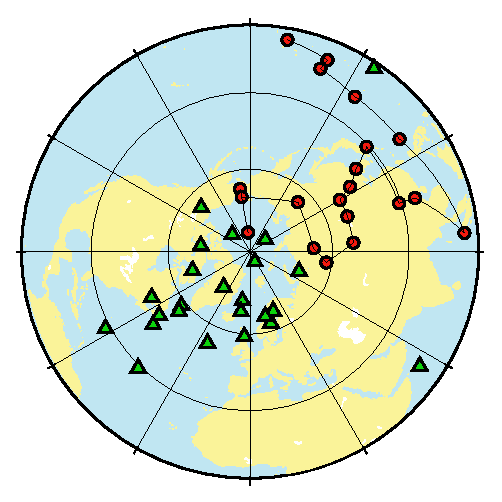
\includegraphics[width=6.5 cm]{EPSfiles/poles_na_dis.eps}
\caption{Circles are ``reliable'' mean poles from 
cratonic North America. (Data as listed in  van der Voo, 1990). So-called
``discordant poles'' from western North America are plotted as triangles. 
[Data from  van der Voo, 1981.]}
\label{fig:poles.dis}
\end{figure} \nocite{voo81}




\begin{figure}[h!tb]
%\epsfxsize 8cm
%\centering \epsffile{EPSfiles/inconly.eps}
 \centering 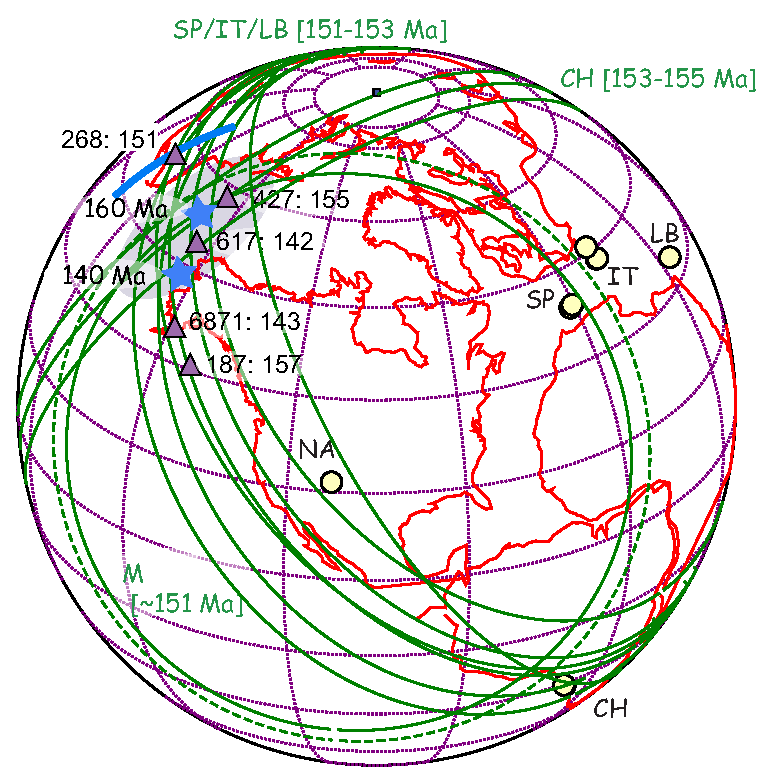
\includegraphics[width=8cm]{EPSfiles/inconly.eps}
\caption{If local rotations are suspected for a given region,  the inclination information can be converted to the equivalent paleo-colatitude small circles (green solid lines) on which the paleopole must lie.  Site locations from `mobile regions'   are shown as open circles.   LB: Lebanon, SP: Spain; IT: Italy; CH: Chile; NA: Morrison Formation on the Colorado Plateau of North America.  Small circles (solid green lines) are the paleomagnetic colatitudes ($\theta$ in Table 16.3) from inclination data.  The dashed line is the paleolatitude from uncorrected inclination data of the Morrison Formation.  Shaded ellipse indicates region of overlap among all small circles.  Fully oriented poles are shown as purple triangles. Numbers are the GPMDB reference numbers followed by the age in Ma.  See Table 16.3. All poles and observation sites have been rotated into South African coordinates for 155 Ma (see Appendix~\ref{app:polerot}) as have the continents.  Pole number 268 is the Canelo Hills Volcanics from Arizona.  If this region rotated about a vertical axis, the pole would lie along the solid blue line.    Blue stars are the predicted poles of Besse and Courtillot (2002) in South African coordinates.    }
\label{fig:inconlypole}
\end{figure}


Use of inclination only data require knowledge of the following:

\begin{enumerate}
\item  The precise age of  the rock unit under study:   This is frequently constrained  by magnetostratigraphy, biostratigraphy or radioisotopic data.
\item (Paleo-)vertical:   Drill cores or ``mobile belts'' often are azimuthally unoriented but the direction to the (paleo-)vertical is known. 
\item Cratonic affiliation:  The allegiance of the rock unit under study to a particular continental fragment or craton must be known in order to rotate the site location into a common reference frame, for example ``fixed South Africa''. 
\item Data from at least three far-flung localities:  One paleolatitude estimate (calculated from the inclination using the dipole formula in Chapter 2) defines  a small circle path around the site location along which the paleopole must lie.  Two such small circles may intersect at two points leaving the true paleopole position ambiguous.  Three far flung locations will intersect at a unique point (see Figure~\ref{fig:triangulation}).   Additional data from fully constrained paleopole positions can be combined with the inclination only data for additional control. 
\end{enumerate}    


We mentioned earlier that
\index{May, S.R.} \index{Butler, R.F.}
May and Butler (1986) \nocite{may86} applied the PEP technique to paleomagnetic poles from North America  (see Figure~\ref{fig:PEP}c), whereby the Jurassic poles (labelled ``G'',``K'', etc. in the figure) were interpreted to fall along small circle segments generated by North American steady plate motion around several Euler poles.   The steady motion, represented by the two tracks labelled ``J1'' and ``J2'' in the figure are separated by a ``cusp'' when the Euler pole shifted positions.    May and Butler (1986) recognized the  problem with the first-order  interpretation of the data shown in Figure~\ref{fig:PEP}c noting that some of the poles may have come from portions of the North American continent that had suffered differential rotation (see Section~\ref{sect:discord}) and they produced a second set of curves that assumed different amounts of rotation for different poles.  Some poles may suffer from sedimentary inclination shallowing as well (see Chapter 7).   In the end, the 
APWP must agree with all the ``reliable'' poles from the continent and the PEP version of the North American  APWP did not agree with several poles from the North American continent considered highly reliable.  It also disagreed with poles that had been rotated into North American coordinates (see, e.g., 
\index{Van Fossen, M.C.}
\index{Kent, D.V.}
Van Fossen and Kent, 1990). \nocite{vanfossen90}     

 The Kimmeridgian poles  listed in Table~\ref{tab:inconly} are plotted as triangles on Figure~\ref{fig:inconlypole} and are poorly clustered.   We can augment the Kimmeridgian data set by allowing 
 data from regions of possible local rotation with respect to the craton using the inclination only technique.  There are many magnetostratigraphic data sets from the Jurassic spanning  the Kimmeridgian from Italy
\index{Channell, J.E.T.}
\index{Vandenberg,    J.}
\index{Wonders, A.A.H.}
 (Channell et al. 1984; 1992; Vandenberg and Wonders, 1976), 
 \index{Ogg, J.G.}
 Spain (Ogg et al. 1984) and the Colorado Plateau 
 \index{Steiner, M.B.}
 \index{Helsley, C.E.}
 (Steiner and Helsley, 1975).  Italy was once part of Africa,  Spain is attached to Europe (after closing of the Bay of Biscay) and the Colorado Plateau is part of the North American continent.  All are known or suspected to have experienced relative rotation with respect to their respective cratonic reference frames.    In addition, there are data  from igneous outcrops in Lebanon 
 \index{Gregor, C.B.}
 \index{van Dongen, P.G.}
 (Gregor et al. 1974; van Dongen et al., 1967) and Chile 
 \index{Randall, D.E.}
 (Randall et al. 1996) that have been dated as  150-155 Ma in age.  Lebanon is part of Africa and Chile, part of South America.  Note that we have not used the  data of Irwin et al. (1987) \nocite{irwin87} because the directions are indistinguishable from the present field and those from 
 \index{Forsythe, R.}
 \index{Chisolm, L.}
 Forsythe and Chisolm (1994) because the normal and reverse data were not antipodal.  \nocite{forsythe94} \nocite{channell84,channell92,vandenberg76,steiner75,randall96,gregor74,vandongen67}    There are a few poles available from stable regions with ages between 140 and 160 Ma, some of which were included in the compilation of 
 \index{Besse, J.}
 \index{Courtillot, V.}
 Besse and Courtillot (2002).   Details of the Jurassic data sets considered here are listed in Table~\ref{tab:inconly}.   

The problem of possible inclination shallowing can be addressed with the so-called elongation/inclination correction method of 
\index{Tauxe, L.}
\index{Kent, D.V.}
Tauxe and Kent (2004; see Section~\ref{sect:tk03}) and local rotations can be treated using the ``inclination-only'' method briefly described in Section~\ref{sect:apwp}.     We focus here on the Kimmeridgian time interval ($\sim$ 151-153 Ma) because there are quite a few paleomagnetic data available, albeit not  all from volcanics in stable cratonic environments.   Indeed, very few poles of this age are included in compilations such as 
\index{Besse, J.}
\index{Courtillot, V.}
\index{Torsvik, T.H.}
Besse and Courtillot (2002) or Torsvik et al. (2008).   We list five poles from the Global Paleomagnetic Data Base 
\index{databases!GPMDB}
(GPMDB) with ages between 143 and 157 Ma.    [NB: One of these is the ``Canelo Hills'' pole from 
\index{Kluth, C.}
Kluth et al. (1982) \nocite{kluth82} which was renamed the ``Glance Conglomerate'' by 
\index{May, S.R.}
\index{Butler, R.F.}
May and Butler (1986),  \nocite{may86}
labeled `G' in Figure~\ref{fig:PEP}.]    



The Morrison Formation is a classic `red-bed' formation. Tuffs at the top and bottom of  the formation have been dated by 
\index{Kowallis, B.J.}
Kowallis et al. (1998) \nocite{kowallis98} and range from 148 Ma to 151 Ma.  Data from this formation have traditionally been divided into Upper and Lower Morrison means (UM  and LM respectively in Figure~\ref{fig:PEP}b), but the short duration of the section suggests that it is unlikely to record significant plate motion and we have lumped all the data together here.  Moreover, because the magnetization is thought to be carried by detrital hematite, notorious for inclination shallowing, we treated the data to the elongation/inclination test described in Section~\ref{sect:tk03}.  The corrected inclination is steeper by about 4$^{\circ}$, insignificantly different from the uncorrected inclination (see Table~\ref{tab:inconly}).  The paleomagnetic colatitude derived from the uncorrected inclination is shown as the dashed line in Figure~\ref{fig:inconlypole},   labelled `M'.    


The paleomagnetic poles from the `mobile' regions must lie along the small circle tracks shown as green lines in Figure~\ref{fig:inconlypole}.  Because there are inclination only data from three quite different regions, labelled CH, NA and  SP/IT/LB, there is a unique crossing point within the shaded region where the paleopole must lie.    This inclination only paleopole for the Kimmeridgian ($\sim 152$ Ma) agrees well with the predicted paleopole from the synthetic APWP of Besse and Courtillot (2002).  The fully determined poles (purple triangles) agree reasonably well with the inclination only data.    Also note that if south eastern Arizona, home to the  Canelo Hills pole (\#268 in Figure~\ref{fig:inconlypole}) suffered rotation like the Colorado Plateau, the unrotated pole would lie along the heavy blue line in Figure~\ref{fig:inconlypole}, which does not improve the fit.  


%

% \begin{figure}[htb]
%\epsfxsize 8cm
%\centering \epsffile{EPSfiles/reference.eps}
%\caption{Reconstruction of Africa at 100 Ma using
%four different frames of reference. Fixed  African
%hot spot predicts significantly more southerly latitudes for
%Africa than all other frames. [Redrawn from Torsvik et al. 2008.]}
%\label{fig:hotspot}
%\end{figure}


%
%\section{Frames of Reference}

%UNDER CONSTRUCTION   Figure~\ref{fig:hotspot}.  

%TALK ABOUT DIFFERENT FRAMES OF REFERENCE - RELATIVE, PALEOMAGNETIC, HOT SPOT, MOVING HOTSPOT, TPW.  I'LL MAKE A FIGURE LIKE YOUR ONE FROM TORSVIK ET AL. 2002 (BUT USING DATA FROM TORSVIK ET AL. 2008) SHOWING POLES IN HOTSPOT REFERENCE FRAME WANDERING AWAY FROM SPIN AXIS.   


\section{Concluding remarks}


And so we return to where we started at the beginning of this book with an assumption that the geomagnetic field is essentially that of a centered dipole.  There is no compelling evidence that the field has operated in a vastly different way in ancient times, apart from the puzzling change in reversal frequency.  We are getting better at all aspects of paleomagnetic research from better designed field programs to better laboratory analyses to more sophisticated data analysis.  There remains much to be done.  Enjoy.


\vskip .25 in\noindent SUPPLEMENTAL READINGS:  Torsvik et al.  (2008). \nocite{torsvik08}

\vskip12pt
\section{Problems}

{\parindent 0pt  \parskip 12pt


{\bf Problem 1}

a) Calculate the expected direction for  about 20 Ma at a locality in the Mojave Desert (latitude of 34.5$^{\circ}$N and longitude  of 117.5$^{\circ}$W).   Use the program {\bf apwp.py}.    Assume that the Mojave  was on the North American Plate.  




b) Go to the MagIC search interface  at: \url{earthref.org/MAGIC/search}.    Click on the search icon and use the `All coordinates are within' filter.   Find the studies from 34.5N 119W to 35.5N 116W.    Once you have applied the search criteria, you will be returned to the Search interface.    Click on the `Locations' and `Paleomagnetics' tabs and save the search (use the `Save As' button).  This will download a file to your desktop.  
Make a new Project Directory  unpack the downloaded file with {\bf QuickMagIC.py}.  

c) Fish out the data that are Neogene in age ($<$30 Ma) and make an equal area  plot of all these results,  Calculate the  average direction, confidence ellipses.   Be sure to only work on single polarity groups. 
How does the average direction compare with the prediction made in Problem 1a?  Explain any differences.  

d) Calculate the VGPs and an average paleopole for these data.  



{\bf Problem 2}

Look back at the Problems for Chapter 15, and use the same data set.  
 What tectonic plate is Site 522 on?  Using the age range inferred from your magnetostratigraphic interpretation and knowing the plate and the present day location,  find the appropriate paleopoles for the top (Oligo/Miocene boundary) and bottom (Eocene/Oligocene boundary) of the dataset from those of  Besse and Courtillot (2002).   \nocite{besse02}
Best and Courtillot (2002) is what is implemented in  the program {\bf apwp.py}  to calculate the  the expected inclinations for the top and bottom  10 meters of the record, respectively.  How do these inclinations compare with the ones in Site 522?  


{\bf Problem 3}


a) Find the appropriate pole of rotation from North America to South African coordinates for 90 Ma (use the right sign for the rotation angle!)  from Appendix~\ref{app:polerot} .

b) Write a program that will transform the North American pole to South African coordinates using the method outlined in the Appendix~\ref{app:polerot}.  The North American pole for 90 Ma  in BC02 is $\lambda=75.2^{\circ}, \phi=201^{\circ}$.   The African pole is $\lambda=66.8^{\circ}, \phi=244.5^{\circ}$.  How does your answer compare? 

{\bf Problem 4}

Find the  data set {\it prob4.dat}  in the Chapter\_16 directory of the Datafiles folder (see Problems for Chapter 5 for instructions in downloading it).  It  
was collected from a study in Spain at a latitude of  41.5$^{\circ}$ and a longitude of  358.5$^{\circ}$ from Miocene aged red bed sediments.  Look up the European pole   for  15 Ma using {\bf apwp.py}.  What is the expected direction at the location for that age?  Make an equal area projection of the data using {\bf eqarea.py}.  What is the average normal and average reverse direction using {\bf eqarea\_ell.py}.  Are these antipodal using, for example {\bf revtest.py}?    

Use the program {\bf tk03.py} to generate a set of directions expected from the statistical field model at that location.  Plot those directions in equal area projection and compare them with the observed directions.  (On a Unix type computer, a handy way to do this would be to pipe the output of {\bf tk03.py} to {\bf eqarea.py}, otherwise save the output of {\bf tk03.py} in a file, then plot it with {\bf eqarea.py}.       

Calculate Bingham ellipses for both data sets using {\bf gobing.py}.   What is different about the two data sets?    (You might have to blow up the error ellipses for a closer look because N is so large......)

Finally, use the  programs  {\bf find\_EI.py} to ``fix'' the data using the E/I method explained in the text.   In the cumulative distribution  plot you have the cumulative distribution of the bootstrap best-fit inclinations and the bounds (in dashed lines).  Is this result consistent with the Besse and Courtillot prediction for this location and age (assume ages of 10 and 20 Ma to get bounds)?   


{\bf Problem 5}

a) Go to the MagIC search interface at: \url{http://earthref.org/MagIC/search}.   click on the Search button and select the following:  Location Contenent or ocean Island Region equals Europe,  Any Age (in Years BP) is between 85,000,000 and 110,000,000,  Any External Database Name equals GPMDB, and Any Method Code contains LP-DC4.  Your web interface should look something like this:

 \centering 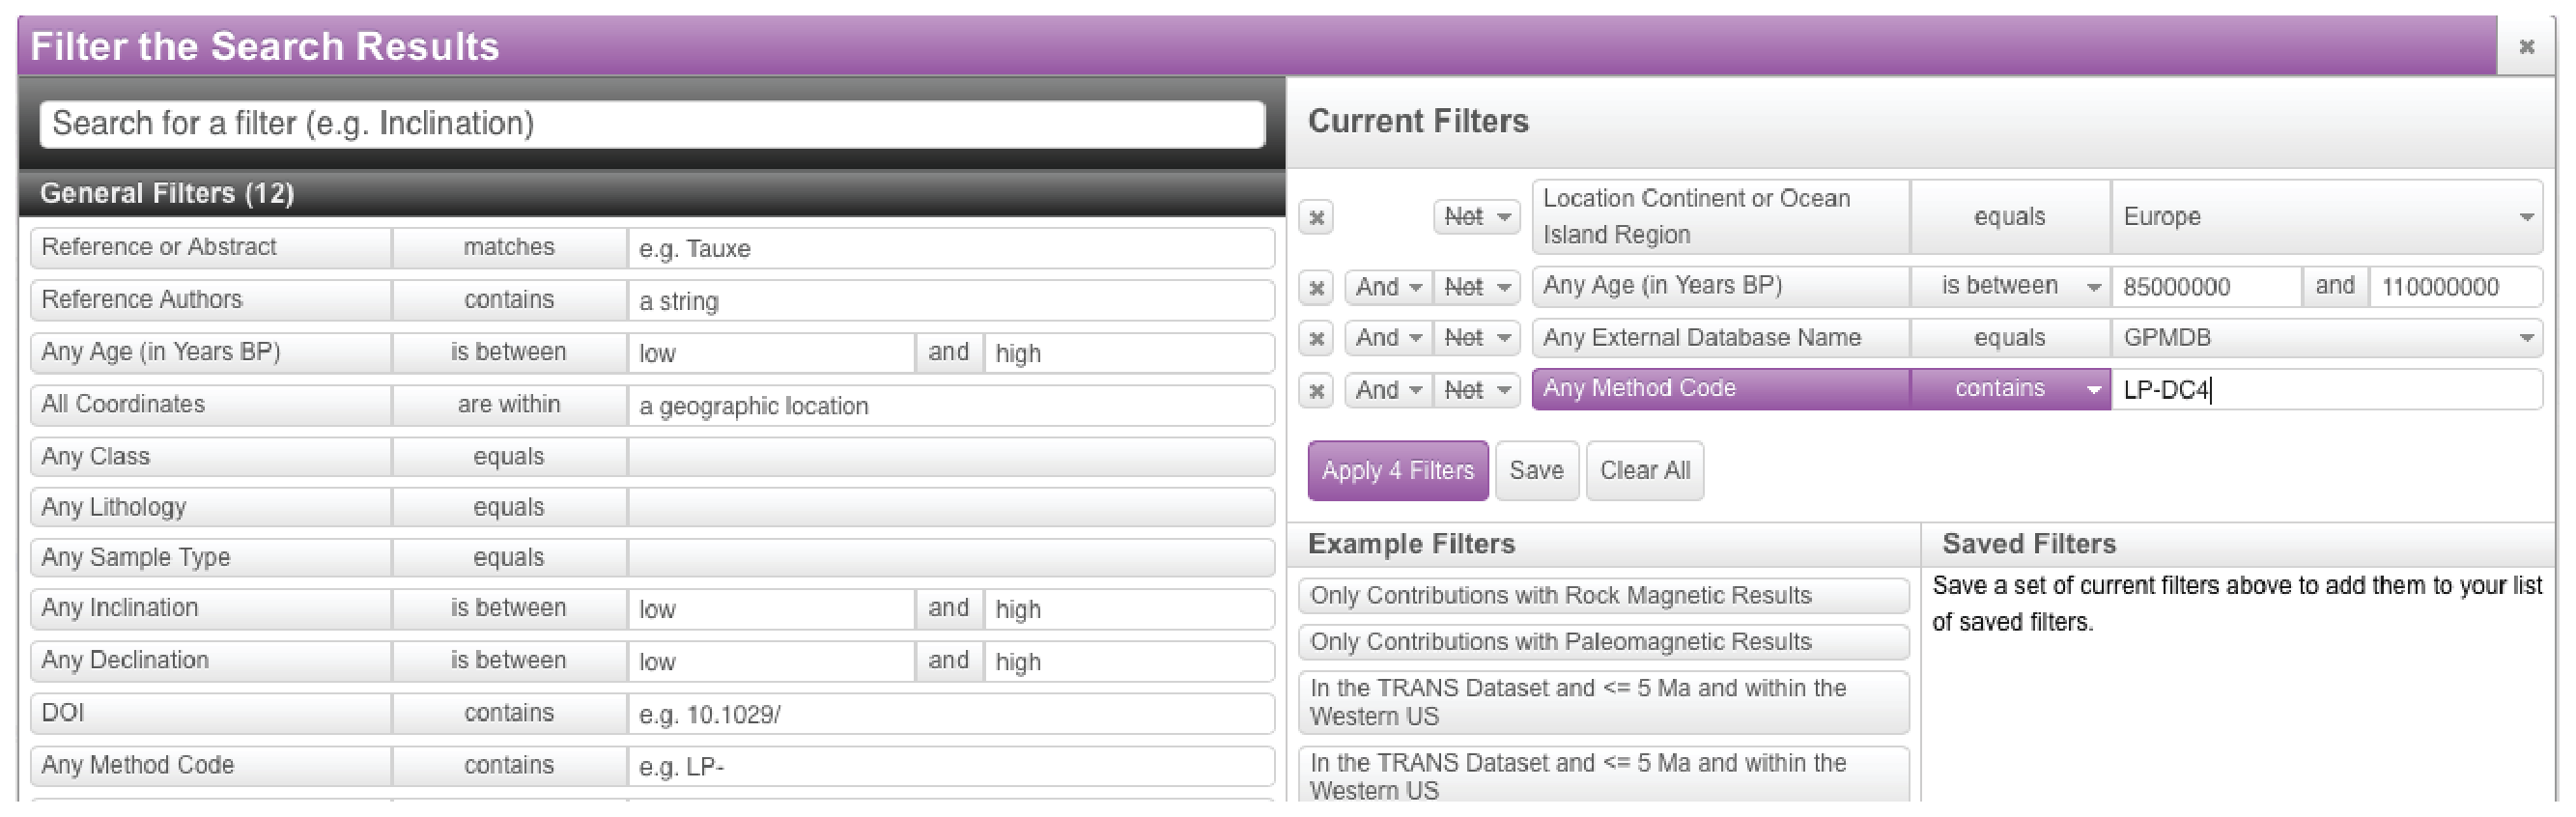
\includegraphics[width=16cm]{EPSfiles/gpmdb_search.eps}
 
 Click on the `Apply 4 filters' button and you will return to the main search interface.  After some time, all the records will be available to you.  Click on the `Locations' tab and then the 'Paleomagnetics' tab.  Then click on the `Save As' button to download your search.  Repeat using a method code of LP-DC5.  
 
 You now have records from the GPMDB (global paleomagnetic data base) database.  The LP-DC4 and LP-DC5 method codes indicate that all the specimens were demagnetized in step wise fashion.    
 
 b) Make a new Project Directory  with two subdirectories (one for each method code) and unpack the two downloaded files (see Problem 1).   Read them into a Pandas DataFrame.  You will notice that our search cast a wide net and there are many results outside the desired age bounds.  You will have to get rid of the ones outside the bounds.  Also, there are a number of suspicious looking 'result_description' fields including words like 'Superseded', 'Overprint', 'Remagnetized', 'Included in RESULTNOS', etc.  Get rid of these too.  



c) Put the pole latitudes and longitudes into a file and use the program {\bf pt\_rot.py} to rotate these to North American coordinates for 100 Ma.  Look up the poles of rotation in Appendix~\ref{app:polerot} for first rotating Europe to fixed African coordinates, then African to North American coordinates (you will have to change the 
 sign of $\Omega$ for the latter).     Save your rotated poles in a file using the '-F' option (creates a MagIC formatted pmag\_results file)  and plot these using the program {\bf vgpmap\_magic.py}.    Or, if you are using IPython notebooks (recommended), you can use the ipmag.plot_vgp function as in Chapter 14.    Compare your rotated pole with the synthetic pole of Besse and Courtillot (2002).  You can find what this is by using the program {\bf apwp.py}.   
 
 d) Make a plot of the continental configurations at 100 Ma using the program {\bf cont\_rot.py}.    Select the European, North American, African, South American, Indian, Australian and Antarctic continents.  



 
 
 }
